%%%%%%%%%%%%%%%%%%%%%%%%%%%%%%%%%%%%%%%%%%%%%%%%%%%%%%%%%%%%%%%%%%%%%%%%%%% 
% 
% Generic template for TFC/TFM/TFG/Tesis
% 
% By:
% + Javier Macías-Guarasa. 
% Departamento de Electrónica
% Universidad de Alcalá
% + Roberto Barra-Chicote. 
% Departamento de Ingeniería Electrónica
% Universidad Politécnica de Madrid   
% 
% Based on original sources by Roberto Barra, Manuel Ocaña, Jesús Nuevo,
% Pedro Revenga, Fernando Herránz and Noelia Hernández. Thanks a lot to
% all of them, and to the many anonymous contributors found (thanks to
% google) that provided help in setting all this up.
% 
% See also the additionalContributors.txt file to check the name of
% additional contributors to this work.
% 
% If you think you can add pieces of relevant/useful examples,
% improvements, please contact us at (macias@depeca.uah.es)
% 
% You can freely use this template and please contribute with
% comments or suggestions!!!
% 
%%%%%%%%%%%%%%%%%%%%%%%%%%%%%%%%%%%%%%%%%%%%%%%%%%%%%%%%%%%%%%%%%%%%%%%%%%% 

\chapter{Predictive Techniques for Scene Understanding in Autonomous Driving}
\label{cha:predictive_techniques_in_ad}

\begin{FraseCelebre}
	\begin{Frase}
		Avanzad, sin temor a la oscuridad. \\
		Luchad jinetes de Theoden. \\
		Caerán las lanzas, se quebrarán los escudos. \\
		Aún restará la espada. \\
		Rojo será el día, hasta el nacer del sol. \\
		Cabalgad, cabalgad, cabalgad hacia la desolación \\ 
		y el fin del mundo. Muerte, muerte, muerte.
	\end{Frase}
	\begin{Fuente}
		Discurso de Theoden, Rey de Rohan \\
		El Señor de los Anillos: El Retorno del Rey
	\end{Fuente}
\end{FraseCelebre}

\section{Introduction}
\label{sec:4_introduction}

\ac{AD} has gained significant attention in recent years, with the development of intelligent vehicles and the increasing need for safe and efficient transportation systems. However, one of the main challenges in the field of \ac{AD} is scene understanding, which involves the ability of a vehicle to recognize and interpret the objects and events in its environment. Accurate scene understanding, particularly focusing on the future behaviour of the scene, is critical for safe and efficient driving, as it enables the vehicle to make informed decisions and take appropriate actions.

\ac{DL} has emerged as a powerful tool for scene understanding in autonomous driving, as it can automatically learn representations of complex and high-dimensional data. In particular, deep neural networks have shown remarkable performance in various tasks related to scene understanding, such as object detection, segmentation, classification or prediction. In that sense, the design and implementation of effective \ac{DL} models for scene understanding is a really active research area, and there is a need for more advanced predictive techniques to improve the performance of autonomous vehicles.

The main scope of this chapter is the development of novel and efficient interaction-aware \ac{DL} based \ac{MP} models, focusing on long-term (from 3 to 6 s) prediction horizon, including social and physical information. Even though the main agent to be predicted will be usually the ego-vehicle, the algorithms proposed in this chapter will be able to properly model the past trajectory and agents interactions based on the specific type of agent, instead of the first \ac{DL} models proposed in the literature which only focused on pedestrian trajectory prediction \cite{alahi2016social, gupta2018social, sadeghian2019sophie}. 

First of all, this chapter will study the incorporation of HD map information to enhance the robustness and reliability of a simple-yet-powerful tracking-by-detection pipeline, based on Kalman Filter and Hungarian algorithm, which subsequently feeds the updated tracker information to perform \ac{CTRV} prediction. Then, \ac{DL} will be progressively integrated to encode the past trajectories, social interactions and physical information respectively, including physics-based heuristics to include map information, specially the potential future goals or centerlines candidates. The goal is to develop advanced models that can accurately recognize and interpret the agents states, interactions and context to provide reliable predictions for safe and efficient driving. 

\section{SmartMOT: Exploiting the fusion of HD maps and Multi-Object Tracking for Real-Time scene understanding}
\label{sec:4_smartmot}

% https://arxiv.org/pdf/2002.04849.pdf
% https://hal.science/hal-03347110/document
% https://www.mdpi.com/1424-8220/22/1/347

One of the key concepts when developing safe \acp{ADS} is the perception of the environment. Furthermore, the reliability of a Collision Avoidance System (CAS) lies on the performance of the environment detector and its ability to predict future situations. In that sense, a real-time \ac{MOT} system, which goal is to associate detections (usually in the 3D or \ac{BEV} space) in a sequence, is essential for \ac{AD} in order to monitor the most important agents around the ego-vehicle. The improvements in object detection in the last years have allowed the research community, specially those groups related to \ac{AD}, to focus on \ac{MOT} techniques as a preliminary stage before implementing \ac{MP}, yielding higher accuracy at the cost of computational cost and complexity, making its use prohibitive in real-time systems. 

\ac{MOT} systems aim to estimate the orientation, location and scale of all the objects in the environment over time. While object detection only captures the information of the environment in a single frame, a tracking system must take temporal information into account, filtering outliers (\aka false positives) in consecutive detections and being robust to partial or full occlusions. When travelling throughout a route programmed by the path-planner, the vehicle may detect an undetermined number of unforeseen objects over which the \ac{MOT} module should consider only the most relevant from a safety point of view (such as pedestrians, cyclists or cars) to predict and monitor their trajectories. Then, the vehicle can use the evolution of the scene over time to infer driving behaviour and motion patters for improved \ac{MP}.

Most \ac{MOT} approaches \cite{weng20203d, chiu2021probabilistic} model the state of each obstacle with its 3D position, scale, orientation and their corresponding linear and angular velocity. These approaches introduce an unnecessary complexity and computational cost to the system since most traffic scenes can be described in terms of 2D position, angular and linear velocity, apart from the orientation and scale of the resulting bounding box, that is, a \ac{BEV} perspective, as depicted in Figure \ref{fig:4_ITSC_2020_coordinates_conversion}. 

\begin{figure}[h]
	\centering
	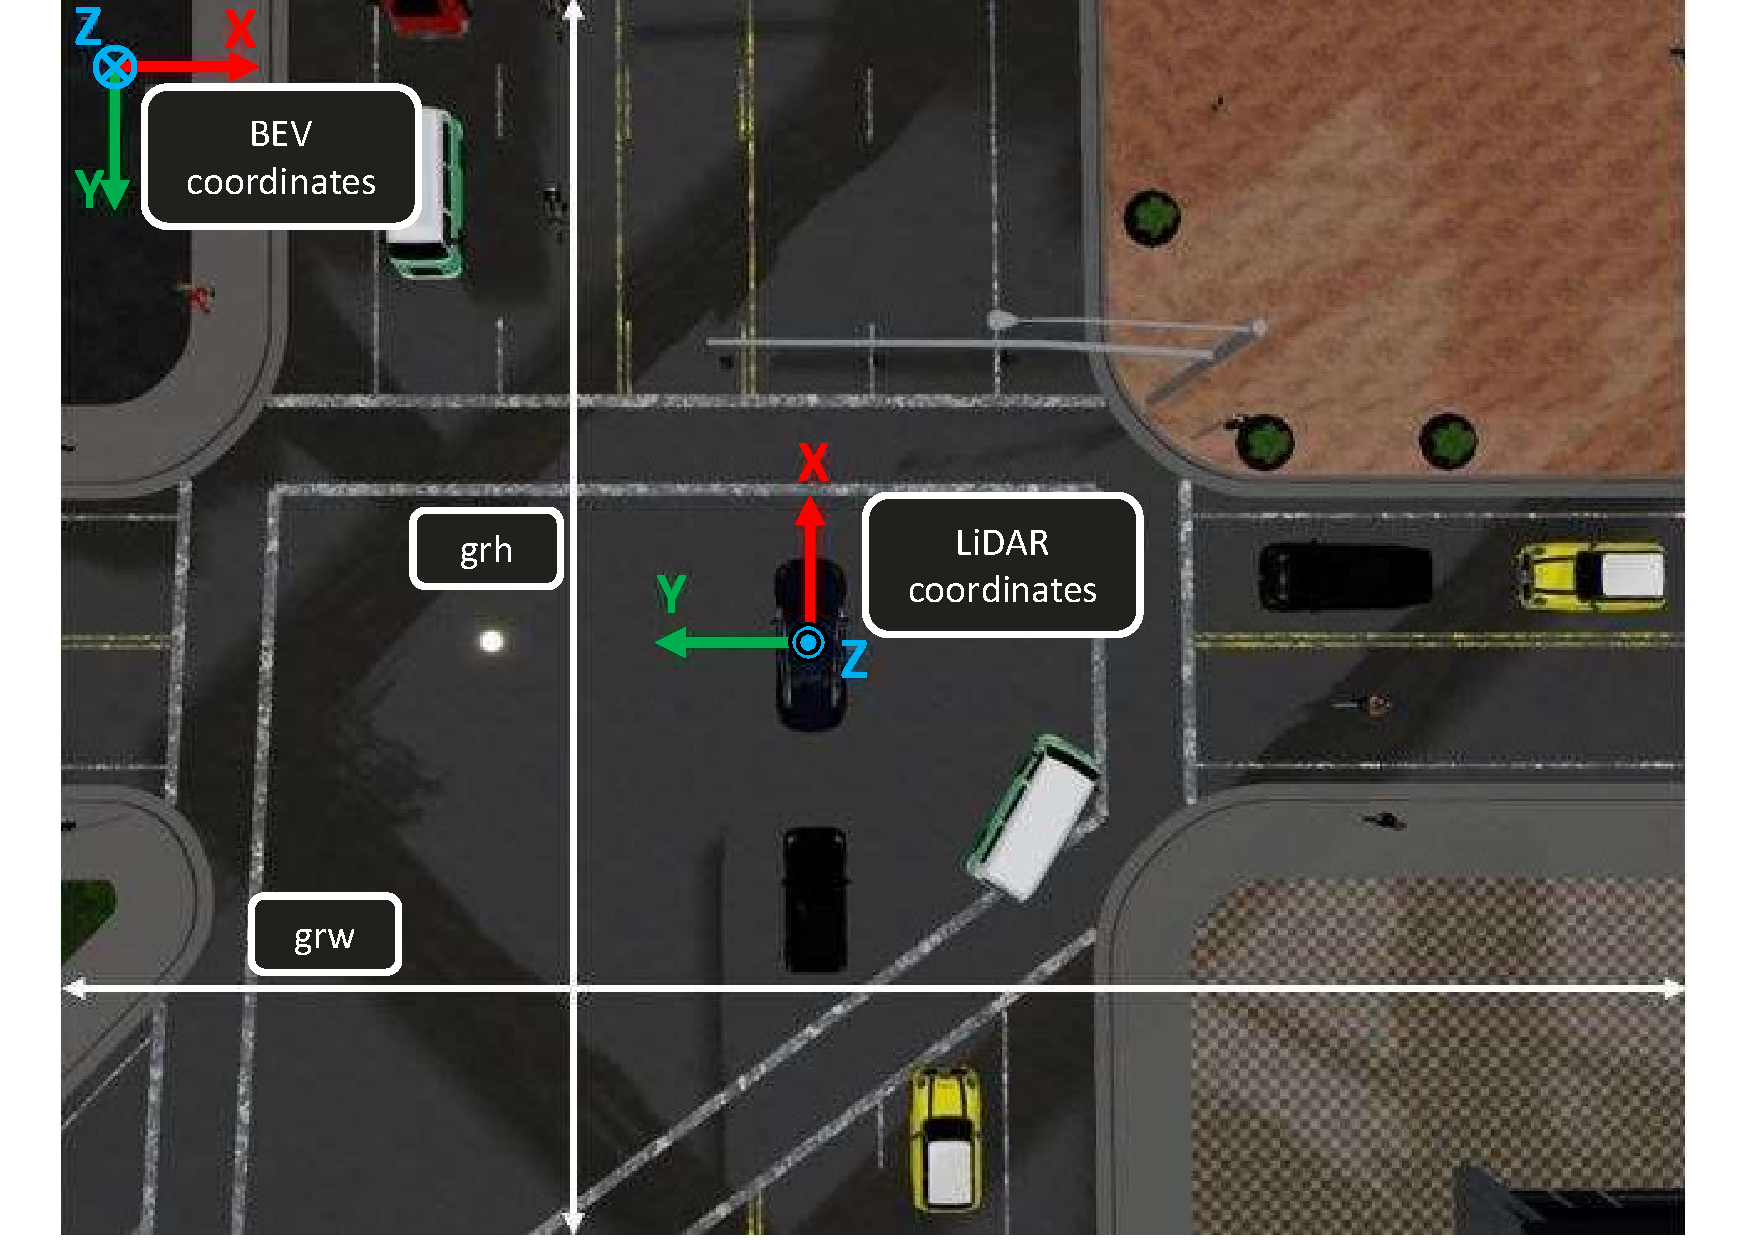
\includegraphics[width=0.42\textwidth]{4_ITSC_2020_coordinates_conversion.pdf}
	\caption{LiDAR to BEV coordinates transformation illustrated in the CARLA simulator}
	\label{fig:4_ITSC_2020_coordinates_conversion}
\end{figure}

In order to solve the problem of monitoring the relevant objects in an efficient way, we propose SmartMOT \cite{gomez2021smartmot}, a simple-yet-accurate combination of traditional techniques such as the Kalman Filter (KF) \cite{kalman1960new} and Hungarian algorithm (HA) \cite{kuhn1955hungarian} for state estimation and data association respectively to solve the tracking-by-detection paradigm. Moreover, as mentioned in Section \ref{sec:4_introduction}, the core interest of SmartMOT is the incorporation of HD map semantic, geometric and topoligical information, in addition to the ego-vehicle status, so as to enhance the efficiency and reliability of the tracking system and subsequent predictions, as observed in Figure \ref{fig:4_IV_2021}. 

The remaining content of this section summarizes the SmartMOT pipeline, being made up by: (1) 3D object detection module that returns the bounding boxes; (2) Monitored Area computation to filter non-relevant objects, \eg the VRUs that are inside the sidewalk far away the road or the vehicles that are located in a lane in which lane change is not allowed, (3) BEV Kalman filter that predicts the object state from the current frame and updates the object state based on the detected bounding boxes at current frame, (4) Hungarian algorithm which associates the current trackers with new detections, (5) Birth and Death memory that deals with the disappeared trajectories (unmatched trajectories exceeding ${age_{max}}$ frames) and the newly appeared trajectories (matched trajectories exceeding ${f_{min}}$ frames) and finally (6) \ac{CTRV} model which performs short-term physics-based motion prediction of the updated trackers information using both the linear and angular velocity information. As observed, except for the pre-trained object detector module (or ground-truth with the corresponding noise, if used), our \ac{MOT} system does not need any training and can be directly used for inference.

\begin{figure*}[thpb]
	\centering
	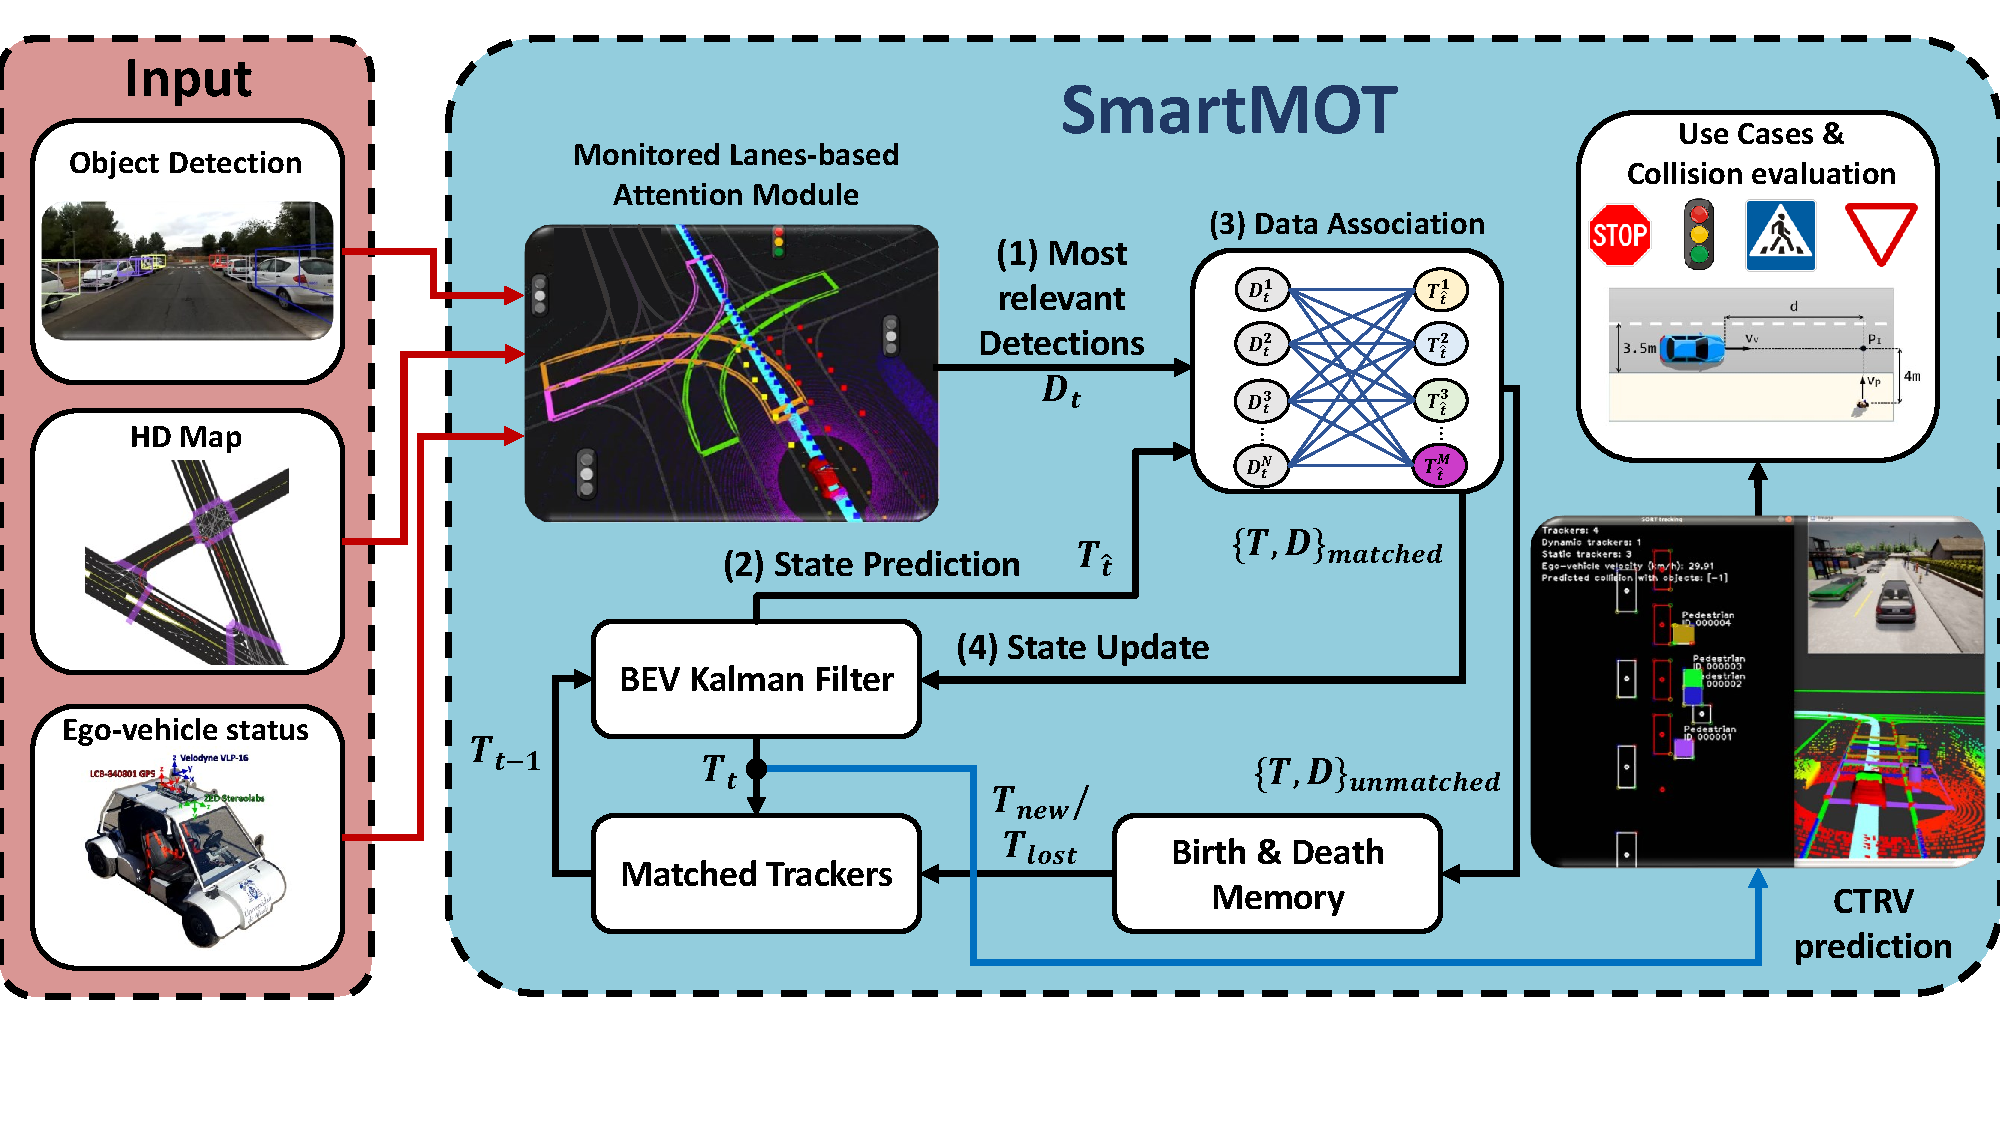
\includegraphics[width=\textwidth]{4_IV_2021.pdf}
	\caption[SmartMOT pipeline]{$\textbf{SmartMOT pipeline}$: $\textbf{(1)}$ The object detection module, mapping layer and localization layer provide the 3D bounding boxes at frame \textit{t}, monitored lanes and ego-vehicle status data respectively; $\textbf{(2)}$ A Monitored Lanes-based Attention Module filters the non-relevant traffic participants and transforms the remaining into the \ac{BEV} image plane; $\textbf{(3)}$ A \ac{BEV} Kalman filter predicts the state of trajectories in frame \textit{t-1} to current frame \textit{\^{t}} throughout the prediction step; $\textbf{(4)}$ detections at frame \textit{t} and predicted trajectories at \textit{\^{t}} are matched using the Khun-Munkres (\aka Hungarian) algorithm; $\textbf{(5)}$ matched trajectories are updated based on their corresponding matched detections and every tracker is evaluated again based on its particular monitorized area, to obtain updated trajectories at frame \textit{{t}}; $\textbf{(6)}$ Unmatched trajectories and detections are used to delete disappeared trajectories or create new ones respectively; $\textbf{(7)}$ Updated trackers at frame \textit{{t}} are predicted using a CTRV model and then evaluated using the monitors module.}
	\label{fig:4_IV_2021}
\end{figure*}

\subsection{3D Object Detection}

The first step our \ac{MOT} algorithm must carry out is to detect the obstacles in the environment around the ego-vehicle. As we will see in Chapter \ref{cha:experimental_results_and_applications}, in order to avoid perspective distortion, we make use of some well known 3D and 2D object detection approaches \cite{lang2019pointpillars, redmon2016you} to perform sensor fusion and retrieve the bounding boxes in the 3D space. Nevertheless, since this thesis do not focus on the object detection stage of the perception layer, some experiments are conducted assuming ground-truth detection including Gaussian noise in the \textit{x,y,z} to simulate real-world detections. Then, at a given frame \textit{t}, the detections provided by the object detection module are given in the following form:

\begin{equation}
	\label{eq:5_smartmot_detection}
	\textbf{D}_{t} =[\textbf{D}_{t}^{1},\textbf{D}_{t}^{2}, ...,\textbf{D}_{t}^{N}]
\end{equation}

Where \textit{N} is the number of detected 3D bounding boxes at a given frame and threshold. At this point, instead of using all the 3D information of the object \cite{chiu2021probabilistic, weng20203d}, we take its projection on the floor plane (\ac{BEV} information), to reduce the complexity and computational cost of the tracking stage, specially in those urban scenarios full of vehicles, based on the assumption that the height (\textit{z}) dimension is not as important as other coordinates (\textit{x}-axis, \textit{y}-axis) in a context of self-driving navigation. Detected 3D bounding boxes are referred to the LiDAR coordinate system. A grid is applied to establish a relation between real-world and image dimensions to discretize the possible positions of the detected bounding boxes and decrease the complexity and computational cost of the tracking module. This grid is featured by a rectangle, whose center is located at the LiDAR position on the vehicle, where $\textit{grw}$ and $\textit{grh}$ represent its width and height in LiDAR coordinates $\textit{m}$ (meters) respectively. Then, each detection in Equation \ref{eq:5_smartmot_detection_tuple} is represented as the tuple:

\begin{equation}
	\label{eq:5_smartmot_detection_tuple}
	\textbf{D}_{t}^{i} = [x_{m},y_{m},w_{m},l_{m},\theta,type,score]
\end{equation}

Where $\textit{$x_{m},y_{m}$}$ correspond to the object centroid in LiDAR coordinates ($\textit{m}$), $\textit{$w_{m}$}$ and $\textit{$l_{m}$}$ correspond to the width and length of the object respectively ($\textit{m}$), $\theta$ its orientation angle around the LiDAR Z-axis, object type and detection confidence. Figure \ref{fig:4_ITSC_2020_coordinates_conversion} illustrates the transformation from the source coordinate system (LiDAR), measured in $\textit{m}$ and placed at the ego-vehicle, to the target coordinate system (BEV), measured in $\textit{px}$ (pixels) and placed on the top-left corner of the grid, which is the most common way to work with images in computer vision. In other words, we deal with the \ac{MOT} problem from the \ac{BEV} image perspective, in order to adapt \ac{MOT} algorithms originally designed for computer vision purposes. 

Equations \ref{eq:5_smartmot_rw_to_image_transform} and \ref{eq:5_smartmot_rw_to_image_apply_transform} show the transformation matrix between both coordinate systems, including both the rotation and the translation (\textit{$\frac{gw}{2}$} and \textit{$\frac{gh}{2}$}), where a $\textbf{LiDAR}_{point}=[x_{m},y_{m},z_{m},1]^{T}$ is given as the column vector in homogeneous coordinates.

\begin{equation}
	\label{eq:5_smartmot_rw_to_image_transform}
	\textbf{T} = \left[ \begin{array}{cccc}
		0  &  -1 &  0  &  \frac{grw}{2} \\
		-1 &  0  &  0  &  \frac{grh}{2} \\
		0  &  0  &  -1 &  0            \\
		0  &  0  &  0  &  1 \end{array} \right] 
\end{equation}

\begin{equation}
	\label{eq:5_smartmot_rw_to_image_apply_transform}
	\textbf{BEV}_{point} = \textbf{T} \cdot \textbf{LiDAR}_{point}
\end{equation}

At this point, each detection is represented by the tuple shown in Equation \ref{eq:5_smartmot_detection_tuple}, but now \textit{$x_{m},y_{m}$} represent the obstacle centroid in \ac{BEV} image perspective. Furthermore, the resolution of the \ac{BEV} image can be modified, in such a way the image width in pixels is given to the algorithm and the image height is calculated according to the aspect ratio of the real world with respect to the width of the image in pixels. Finally, to convert a point from real-word units ($\textit{m}$) to camera units ($\textit{px}$), we apply the corresponding scale factor to each coordinate:

\begin{equation}
	\label{conversion}
	\left[ \begin{array}{c}
		x_{px}  \\
		y_{pc} \end{array} \right] 
	=
	\left[ \begin{array}{cc}
		\frac{gpw}{grw} & 0  \\
		0 & \frac{gph}{grh} \end{array} \right]
	\left[ \begin{array}{c}
		x_{m}  \\
		y_{m} \end{array} \right] 
\end{equation}

However, it is very common to have different scales for $\textit{x}$ and $\textit{y}$-axis since it is more interesting to have a further view in the $\textit{x}$ LiDAR axis rather than a large side sweep in terms of $\textit{y}$ LiDAR axis. Considering this hypothesis, the right way to obtain the width and length of the \ac{BEV} LiDAR bounding box in $\textit{pixels}$ is to obtain the corners of the rotated bounding box in pixels and then compute the \textit{L2} (\aka Euclidean distance) among the corresponding corners to obtain the width and length in $\textit{pixels}$. Nevertheless, the object detector provides the rotation angle of the obstacle (featured as $\theta$) according to its own coordinate system and not around the ego-vehicle coordinate system. Regarding this constraint, to calculate the dimensions of the bounding box in pixels, three steps must be followed:

\[
c1_{m} = (x_{m}-\frac{l_{m}}{2},y_{m}-\frac{w_{m}}{2}) \]
\[
c2_{m} = (x_{m}-\frac{l_{m}}{2},y_{m}+\frac{w_{m}}{2}) \]
\[
c3_{m} = (x_{m}+\frac{l_{m}}{2},y_{m}-\frac{w_{m}}{2}) \]
\[
c4_{m} = (x_{m}+\frac{l_{m}}{2},y_{m}+\frac{w_{m}}{2}) \]

First, we assume a horizontal bounding box ($\theta$ = 0) at the BEV image coordinate system origin, where $\textit{c1}$ corresponds to the top-left corner ($\textit{c2}$, $\textit{c3}$ and $\textit{c4}$ are placed clockwise). Then, using the above equations for each corner, the Euclidean distance is applied between $\textit{c1}$ and $\textit{c2}$ to obtain the width in pixels, in the same way that the Euclidean distance is applied between $\textit{c1}$ and $\textit{c4}$ to obtain the length in pixels.

\begin{equation}
\label{widthpixels}
w_{px} = \sqrt{(c1_{px,x}-c2_{px,x})^2 + (c1_{px,y}-c2_{px,y})^2}
\end{equation}

\begin{equation}
\label{lengthpixels}
l_{px} = \sqrt{(c4_{px,x}-c2_{px,x})^2 + (c4_{px,y}-c2_{px,y})^2}
\end{equation}

Finally, the first four variables of the detection tuple shown in Equation \ref{eq:5_smartmot_detection_tuple} are converted into pixels, in such a way the tracking algorithm will monitor these bounding boxes in the BEV image by using the following tuple:

\begin{equation}
	\label{detpx}
	\textbf{D}_{t,i} = [x_{px},y_{px},w_{px},l_{px},\theta,type,score]
\end{equation}

\subsection{Monitored Lanes-based Attention Module}
\label{subsec:4_smartmot_mlam}

\acp{ADS} need to locate itself in the environment to know what is happening around in order to make decisions and execute a correct navigation like a human driver would. When we talk about localization, the first thing we need is a map where to be located and, particularly for vehicles, this is road map. Road maps used by current navigators, \eg Google Maps, are not valid for AV because of data type and the fact that they are not accurate enough to be used for autonomous driving. Here is where HD maps appear to solve this problem.

A HD map is usually a text file describing the real-world features related to the road map and its location within a 2D/3D space, and can do things that other sensors cannot \cite{wong2020mapping}: First, they have an \textit{infinite range} and, therefore, can \textit{see} even into occluded areas. Second, HD maps will never fail due to environmental conditions. Lastly, HD maps contain highly refined data. This information can be used by different modules of an AV, (including localization, vehicle control, path planning, perception and system management) drastically reducing the computational load and complexity in comparison to other more complex methods, providing robustness and reliability to the system.

\begin{figure}[] 
	\centering
	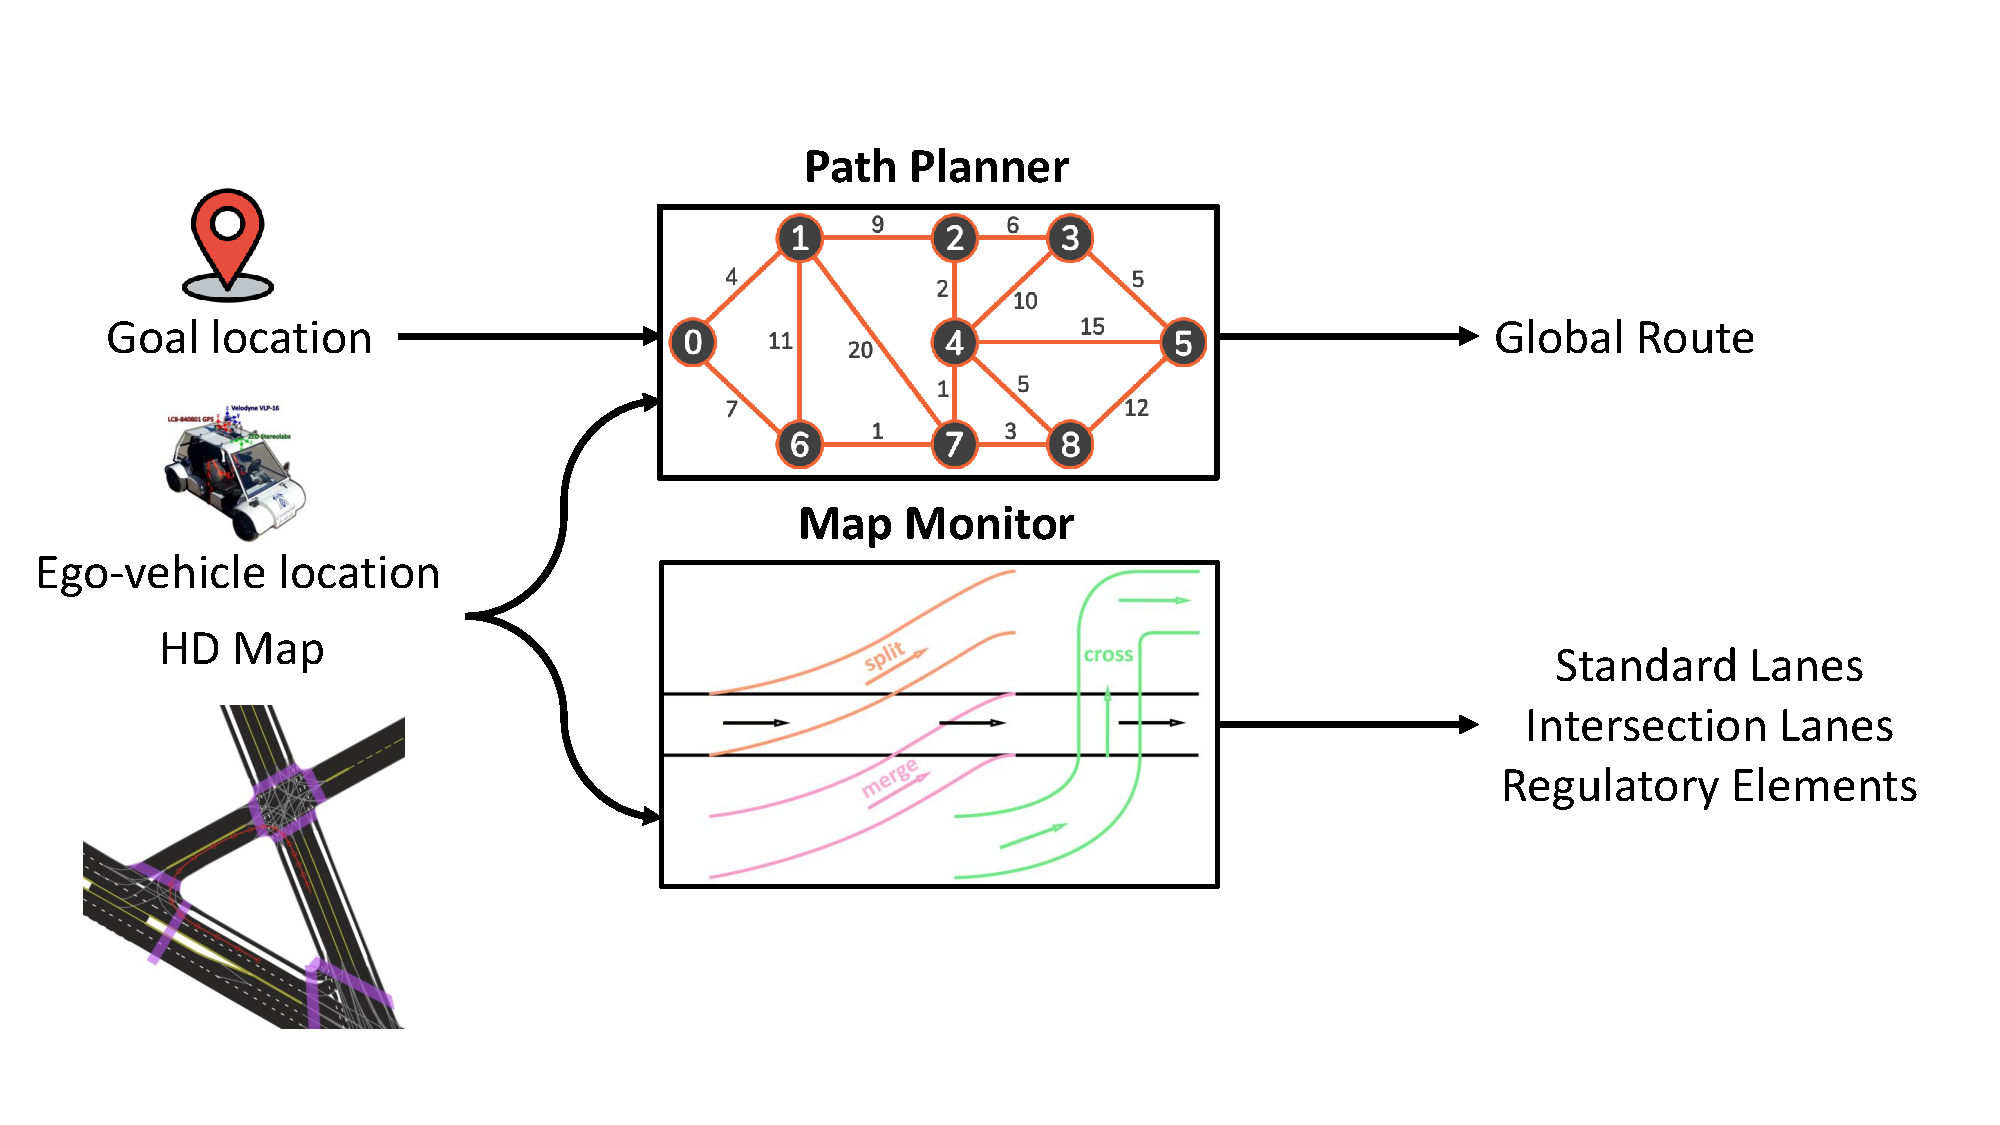
\includegraphics[width=0.8\textwidth]{4_path_planner_map_monitor.pdf}
	\caption{Path Planning and Map Monitoring Outline}
	\label{fig:4_path_planner_map_monitor}
\end{figure}

In terms of mapping information, we may distinguish three main categories:

\begin{itemize}
	\item Topological information provides the connectivity between geometry features. Particularly in the field of \ac{AD}, this is usually the network of roads. This kind of information can allow vehicles to traverse the most energy-efficient route, based on traffic speed, road grade or distance, as well as ensure that \acp{ADS} obey traffic regulation orders, such as one-way streets or the corresponding regulatory elements (pedestrian crossing, traffic light, stop signal, etc.).
	\item Geometric information provides the geometry or shape of other environmental features which can be static (permanent obstruction, such as buildings, bridges or tunnels), temporary (exist for only a limited amount of time, like traffic cones, parked vehicles or temporary road works) and dynamic features (moving people, objects or vehicles). Most of these features are incorporated by means of perception systems, specially in terms of dynamic features, in order to include that information in the HD map for successful motion planning and prediction.
	\item Semantic information returns the \textit{meaning} of aforementioned features, such as road speed limit, road classification, lane information or even the relational information among the different lanes, \ie how lanes work together, different types of lanes, where vehicles must stop and where vehicles can and cannot turn.
\end{itemize}

As illustrated, providing rich physical contextual information allows \acp{ADS} to make informed decisions in different driving scenarios. In our group, we particularly make use of the OpenDrive \cite{dupuis2010opendrive} HD map format, which has been mainly used for two different purposes, as shown in Figure \ref{fig:4_path_planner_map_monitor}:

\begin{itemize}
	\item Global Path Planning, which uses a specific path planner which inputs are the HD map information and the ego-vehicle current location to retrieve an optimal (usually optimized based on the travelled distance) global route towards an specific goal.
	\item Map monitoring, responsible for monitoring the most relevant static and dynamic map elements around the ego-vehicle at each timestep, such as standard lanes (current, back), intersection lanes (merge, split and cross) and regulatory elements (e.g. give way, stop, pedestrian crossing, traffic light).
\end{itemize}

In particular, given a pre-defined global route, in this thesis we focus our interest on designing a map monitor module, responsible for retrieving the most relevant lanes around the ego-vehicle to enhance real-time perception and scene understanding requirements.

\subsubsection{Map Monitor}
\label{subsubsec:4_smartmot_mapmonitor}

The Map Monitor module is in charge of monitoring the surrounding area of the vehicle. The inputs of the Map Monitor are the information provided by the Map Parser module (in charge of getting the information of the map from the HD map file and transform it into custom classes that can be used by other modules like Planning or Perception) and the waypoint route previously obtained by the path planner. The main goal of the Map Monitor is to only monitor the most relevant map elements around the ego-vehicle given the route provided by the global planner (or a new route if the local planer decides to recalculate the route). 

First, the path planner returns the route which is divided in segments separated by a given distance and calculates in which segment of the route the ego-vehicle is found, activating a flag in such a way the Map Monitor can start operating. Otherwise, in case the ego-vehicle cannot be located inside the route, the Map Monitor is deactivated. Secondly, a monitor callback is called periodically every time the ego-vehicle status (position, velocity, orientation, etc.) is received, as observed in Figure \ref{fig:4_IV_2021}. This callback evaluates, if the Map Monitor module is active, calculates the monitored elements frontwards and backwards for a given distance which is proportional to the ego-vehicle velocity given a braking distance linear model that establishes a linear regression between two arrays of velocity and braking distance data. Nevertheless, we make use of a threshold distance to avoid not monitoring if the ego-vehicle is stopped. We will detail the corresponding hyperparameters in Chapter \ref{sec:5_mot_and_euroncap}.

The monitored elements are:

\begin{itemize}
	\item \textbf{Standard Lanes}: Current, back and the corresponding left and right lanes. Current lane is monitored from current position to a dynamic distance depending on the velocity of the ego-vehicle. Back lane is monitored from current position to back a proportional distance of the dynamic current lane obtained distance. Left and right lanes are monitored the same distance that current and back only if the lane marking from the HD map data allows the lane change.
	\item \textbf{Intersection Lanes}: Other lanes that intersect the current monitored lane are checked. Intersection lanes can have different roles: split (1 lane splits into 2 or more), merge (2 or more lanes merge into 1) and cross (a lane crosses a part of the current lane). To calculate the intersection lanes, each lane of every junction (junctions are areas where more than 2 roads meet) in the current lane is evaluated. The polygon of each lane is calculated and evaluated if is inside the polygon of the current lane. It is important to consider that roundabouts are considered as a set of multiple junctions. 
	\item \textbf{Regulatory Elements}: The monitored elements are stops, giveaways, traffic lights, speed limits and crosswalks. The regulatory elements are only monitored for the next intersection affecting the route. 
\end{itemize}

An example of our map monitor module in the CARLA simulator \cite{dosovitskiy2017carla} using the ROS \cite{quigley2009ros} visualizator (R-VIZ) may be observed in Figure \ref{fig:4_monitored_area_CARLA_ROS}:

\begin{figure}[!ht] 
	\centering
	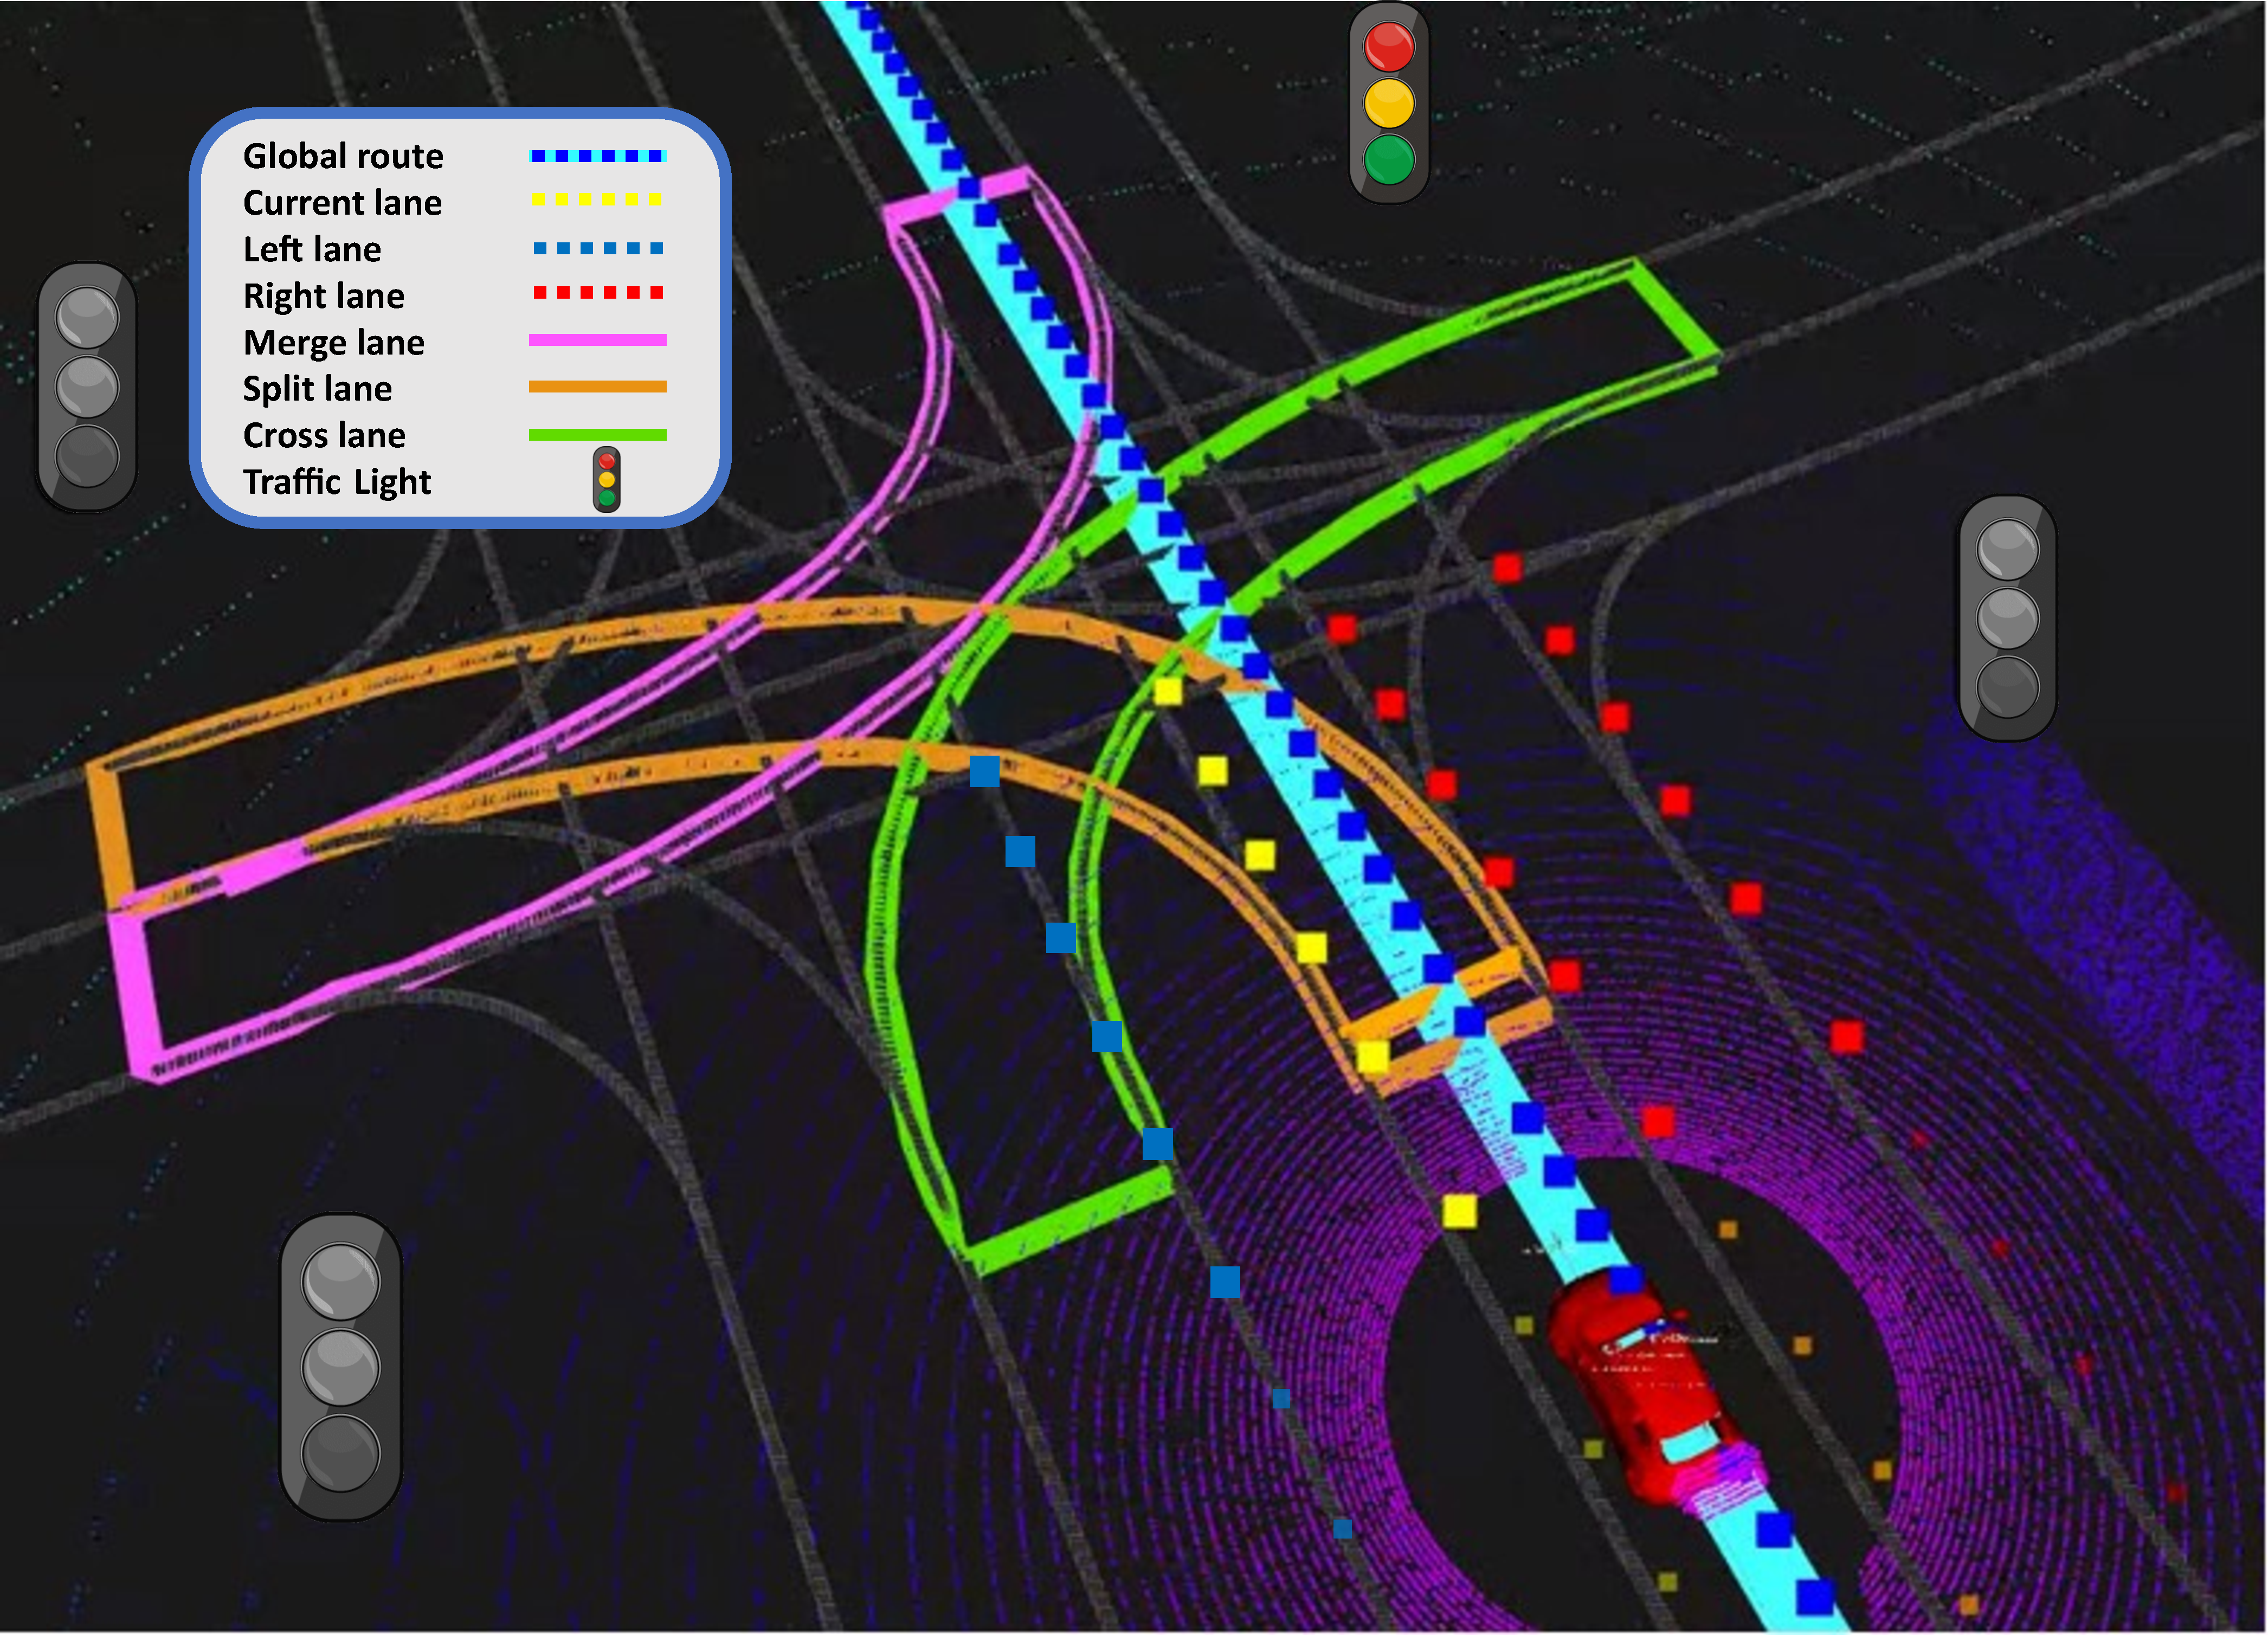
\includegraphics[width=0.8\textwidth]{4_lane_types.pdf}
	\caption[Monitored area in the CARLA simulator using ROS visualizator (R-VIZ)]{Monitored area in the CARLA simulator using ROS visualizator (R-VIZ). It can be appreciated the visualization of the global route, standard lanes, intersection lanes and different traffic lights (regulatory elements). Note that the relevant traffic light is coloured while remaining ones are masked.}
	\label{fig:4_monitored_area_CARLA_ROS}
\end{figure}

As illustrated in Figure \ref{fig:4_IV_2021}, once the object detections have been provided and the monitored area has been computed, the Monitored Lanes-based Attention Module helps us to increase the efficiency and robustness of the system to avoid tracking and predicting all obstacles in the environment, which would escalate the computational cost especially in arbitrarily complex urban scenario. This attention module is not focused on \ac{DL} since the main purpose is to filter non-relevant obstacles in an efficient and interpretable way, such as agents driving way in opposite direction lanes, parked vehicles or pedestrians who are chatting on the sidewalk. The filtering process carried out by our Monitored Lanes-based Attention Module is summarized as follows:

\begin{algorithm}[H]
	\SetAlgoLined
	\KwData{point, polygon}
	\KwResult{isInside}
	crossings $\leftarrow$ 0\;
	\For{i from 0 to (polygon.length - 1)}{
		vertex1 $\leftarrow$ polygon[i]\;
		vertex2 $\leftarrow$ polygon[(i + 1) mod polygon.length]\;
		\If{(point.y > min(vertex1.y, vertex2.y)) \textbf{and} (point.y $\leq$ max(vertex1.y, vertex2.y))}{
			\If{point.x $\leq$ max(vertex1.x, vertex2.x)}{
				\If{vertex1.y $\neq$ vertex2.y}{
					xIntersection $\leftarrow$ (point.y - vertex1.y) * (vertex2.x - vertex1.x) / (vertex2.y - vertex1.y) + vertex1.x\;
					\If{vertex1.x == vertex2.x \textbf{or} point.x $\leq$ xIntersection}{
						crossings $\leftarrow$ crossings + 1\;
					}
				}
			}
		}
	}
	isInside $\leftarrow$ (crossings \% 2 == 1)\;
	\KwRet{isInside}\;
	\caption{Jordan's Curve theorem to determine if a point is inside a polygon}
	\label{alg:4_jordan_curve_theorem}
\end{algorithm}

\begin{enumerate}
	\item First, we determine the lanes of interested around the vehicle, till a given threshold. The minimum information will be the current front and back lane information (mandatory for the Adaptive Cruise Control and Unexpected Pedestrian use cases), as well as left and right lane information if lane change is available considering the presence of a discontinuous line. Moreover, if an intersection is near the ego-vehicle, other lanes of interest such as merging, splits and intersections are considered, which are specially useful in urban scenarios when the vehicle faces a roundabout or other vehicles incorporation in an intersection.
	\item In order to consider an agent as relevant, we study the presence of this agent in our monitored lanes in an elegant and efficient way. The main idea is to find the polygon segment (two nodes on the left, same on the right) closest to the agent. To do that, we iteratively compute the \textit{L2} distance between the agent position (transformed into global (\aka map) coordinates) and the left way nodes (starting from the beginning) of a certain lane. Note that it is irrelevant to take either the left or right lane in terms of observing if the detection is inside a polygon made up by four nodes of the lane, such as there exists the same number of nodes for both ways. For example, in the case of an agent located in front of the vehicle, the distance will decrease since the subsequent left way nodes are closer to the agent. 
	\item Once the new calculated distance is greater than the previous value, that means the closest segment with nodes \textit{$N_0$} and \textit{$N_1$} are found. Taking the same lane indexes in the right way, we obtain a 4-side polygon in which the detection is evaluated using the Jordan curve theorem \cite{tverberg1980proof}, as depicted in Algorithm \ref{alg:4_jordan_curve_theorem}. In this theorem, the input parameters are a point and a polygon, where, by means of a simple-yet-accurate ray casting algorithm, a loop is used to iterate over the polygon vertices and performs the necessary checks to determine the number of crossings. The Jordan's Curve Theorem states that a point is inside a polygon if the number of crossings from an arbitrary direction is odd. Consequently, in our particular case, if the object detection lies outside the closest polygon segment, the traffic participant is considered as non-relevant.
	\item Nevertheless, despite this proposal is coherent for non-holonomic obstacles with more constrained behaviours like cars, vans or trucks, the behaviour of Vulnerable Road Users (VRUs), such as pedestrians or cyclists, is usually difficult to predict. Hence, we widen the closest segment area a certain threshold \textit{L} to the sidewalk so as to track the closest VRUs to the road.
\end{enumerate}

\subsection{BEV Kalman Filter: State Prediction}
\label{subsec:4_smartmot_state_prediction}

Once we have obtained the most relevant \ac{BEV} detections of the environment, a \ac{BEV} Kalman Filter is used to track the objects. To predict the state of object trajectories from the previous frames to the current frame, we approximate objects inter-frame displacement using a constant velocity model which is independent of other objects in the scene and of the LiDAR motion. Regarding this, the estimation of the measured variables in the following frame are:

\[
x_{px}(\hat{t})=x_{px}(t)+v_{x} \:\:\:\:\:\: ; \:\:\:\:\:\: y_{px}(\hat{t})=y_{px}(t)+v_{y}\]
%\[
%y_{px}(\hat{t})=y_{px}(t)+v_{y} \]
\[
s(\hat{t})=s(t)+v_{s} \:\:\:\:\:\: ; \:\:\:\:\:\: 
\theta(\hat{t})=\theta(t)+v_{\theta}\]
%\[
%\theta(\hat{t})=\theta(t)+v_{\theta} \]

Since we formulate the tracking problem over the \ac{BEV} plane, we remove all variables related to the third dimension of the object, such as its $\textit{z}$ coordinate of the 3D bounding box centroid, its associated velocity and the height of the obstacle. On the other hand, since our tracking-by-detection algorithm is inspired by the well-established SORT (Single Online and Real Time) \cite{bewley2016simple} tracking model, originally proposed to track pedestrians using videos as input, some additional variables are included in the object state, such as the aspect ratio and the scale of the bounding box. The aspect ratio can be defined as the relation between the width and the length of the obstacle. Likewise, the scale represents the area of the target bounding box. Then, the state of each object tracker (usually referred as trajectory tracker in the literature) can be expressed as:

\begin{equation}
	\label{state}
	\textbf{T}_{t}^{j} = [x_{px},y_{px},s,r,\theta,x_{px}^{'},y_{px}^{'},s^{'},\theta^{'}]
\end{equation}

Note that the angular velocity $\theta^{'}$ is used in the state space to improve the prediction of the obstacle in later frames. Furthermore, as shown in \cite{bewley2016simple}, the aspect ratio of the bounding box is considered to be constant. As observed in Figure \ref{fig:4_IV_2021}, at every frame \textit{t}, a tuple $\textbf{T}_{t}=[\textbf{T}_{t}^{1},\textbf{T}_{t}^{2}, ...,\textbf{T}_{t}^{M}]$ is returned by the data association module, where each element correspond to an association between a detection and a tracker. Note that $M$ represents the current number of trackers. Then, based on these associations between trackers of the previous frame and current detections, and assuming a Kalman Filter of first order (constant velocity model), the tuple $\textbf{T}_{\hat{t}}$ is calculated, where each element corresponds to the predicted trajectory ($\textbf{T}_{\hat{t}}^{j}$) in the current frame $\textit{t}$ expressed as:

\begin{equation}
	\label{est}
	\textbf{T}_{\hat{t}}^{j} = [x_{px}(\hat{t}),y_{px}(\hat{t}),s(\hat{t}),r,\theta(\hat{t}),x_{px}^{'},y_{px}^{'},s^{'},\theta^{'}]
\end{equation}

This tuple of predicted trajectories based on the previous frame associations, in addition to the current frame detections, represents the inputs to the data association algorithm at frame $t$.

\subsection{Data association}

In order to associate the detections $\textbf{D}_{t}$ and the trackers information after the Kalman Filter state prediction $\textbf{T}_{\hat{t}}$, the Hungarian algorithm is applied. The resulting affinity matrix presents $N$ rows (number of detections at frame $t$) and $M$ columns, which correspond to the number of predicted trajectories based on the information of frame $t-1$. Each element of the matrix corresponds to the Intersection over Union (IoU) in the \ac{BEV} plane between every pair of predicted trajectory and detection. Then, following the principles stated in Algorithm \ref{alg:3_ha}, we solve the bipartite graph matching problem, rejecting the matching if the BEV-IoU metric is lower than a given hyperparameter $IoU_{th}$, giving rise to a set of matched detections ($\textbf{D}_{matched}$) and predicted trackers ($\textbf{T}_{matched}$) with the same length $H$ (the number of matches), as well as a set of unmatched detections ($\textbf{D}_{unmatched}$), where $P = N - H$ is the number of unmatched detections, and a set of unmatched trajectories ($\textbf{T}_{unmatched}$), where $Q = M - H$ is the number of unmatched detections.

\subsection{BEV Kalman Filter - Object State Update}

As observed in Figure \ref{fig:4_IV_2021}, once we have the corresponding sets of matched detections and trajectories, based on the Kalman Filter prediction-update cycle, we update the state space of each trajectory based on its corresponding matched detection. To do that, we use the weighted average between the matched detection values and the state space of the trajectory tracker, according to \cite{kalman1960new}. 

On the other hand, in the same way that \cite{weng20203d}, we appreciate that this state update step does not work properly for obstacle orientation. The reason is simple: Unless the object detector is based on sensor fusion and vision information is included, the object detector cannot distinguish if the obstacle is rotated 0 or $\pi$, $\frac{\pi}{2}$ and $\frac{3\pi}{2}$, and so on, around its \textit{z}-axis. That is, the orientation may differ by $\pi$ in two consecutive frames. Then, if no orientation correction is applied, the Kalman Filter associated to the tracker can get easily confused, since it tries to adapts itself to the new orientation value rotating the object by $\pi$ in following frames, giving rise to a low BEV-IoU between new detections and predicted trajectories. However, regarding the assumption that obstacles must move smoothly and its orientation cannot be modified by $\pi$ in one frame (0.02 s assuming a frequency of 10 Hz), when this happens the orientation of the corresponding matched detection or matched tracker can be considered wrong. To solve this problem, the detection module only considers angle from 0 to $\pi$ (that is, if an angle exceeds $\pi$, it is substracted to the provided angle). Moreover, if the difference of orientation between a given matched detection and its corresponding matched trajectory is greater than $\frac{\pi}{2}$, as stated before, either the orientation of the detection or the orientation of the tracker is wrong. Finally, we add $\pi$ to the orientation of the tracker with the aim to be consistent with the matched detection. 

\subsection{Deletion and Creation of Track Identities}

When obstacles leave and enter the aforementioned monitored lanes, unique identities must be destroyed or created accordingly. In most tracking algorithms it is known as the Birth and Death Memory, which is based on the set of unmatched trackers and detections provided by the data association algorithm, where the unmatched trackers represent potential objects leaving the monitored area, in the same way that unmatched detections represent potential objects entering in the area of interest. 

In order to avoid tracking of false positives or non-relevant obstacles, a new tracker is not created until the unmatched detection has been continuously detected in the next $f_{min}$ frames. Then, the tracker is initialized with the features of the detected bounding box, and the associated velocities set to zero. Note that, as stated in \cite{bewley2016simple}, since the velocity associated to the measured variables is unobserved at this moment (i.e., tracker initialization), the covariance initializes the value of the velocities (in the present work, velocity of the $x_{px},y_{px}$ centroid, scale $s$ and rotation angle $\theta$) with large values, reflecting their uncertainty. 

To avoid removing true positives trajectories from the scene, they are not terminated unless they are not detected during consecutive $a_{max}$ frames. This assumption prevents an unbounded growth in the number of localisation errors and trackers due to predictions over long duration where the object detector does not provide any correction. Note that since this work does not consider object re-identification for simplicity, an object should leaves the scene and then reappers, according to the SORT algorithm, if it is initialized with a new tracker under a new identity. As shown in Figure \ref{fig:4_IV_2021}, the inputs to the Matched Trackers module are the updated matched trajectories from the BEV Kalman Filter and a set of created and deleted trackers, which jointly represent the input trajectories for the prediction step in the following frame.

\subsection{CTRV prediction}
\label{subsec:4_smartmot_ctrv_prediction}

The last stage of our SmartMOT pipeline is a physics-based \ac{MP} model to predict the future behaviour of the agents in the short-term. In particular, we make use of the previously studied \ac{CTRV} model. Once the tracker information (position, velocity and orientation) has been retrieved in real-world coordinates (instead of \ac{BEV} image coordinates), we are able to differentiate between static and dynamic agents. Then, given the ego-vehicle status and dynamic agents short-term prediction, we are able to analyze the risk of collision or to carry out the state of the current behaviour (Adaptive Cruise Control, Pedestrian Crossing, etc.) in such a way SmartMOT can send a signal to suddenly stop the car. Further experiments will be detailed in Chapter \ref{sec:5_mot_and_euroncap}. Figure \ref{fig:4_filtering_process_example} illustrates an example of the filtering process, tracking-by-detection paradigm and \ac{CTRV} prediction.

\begin{figure}[] 
	\centering
	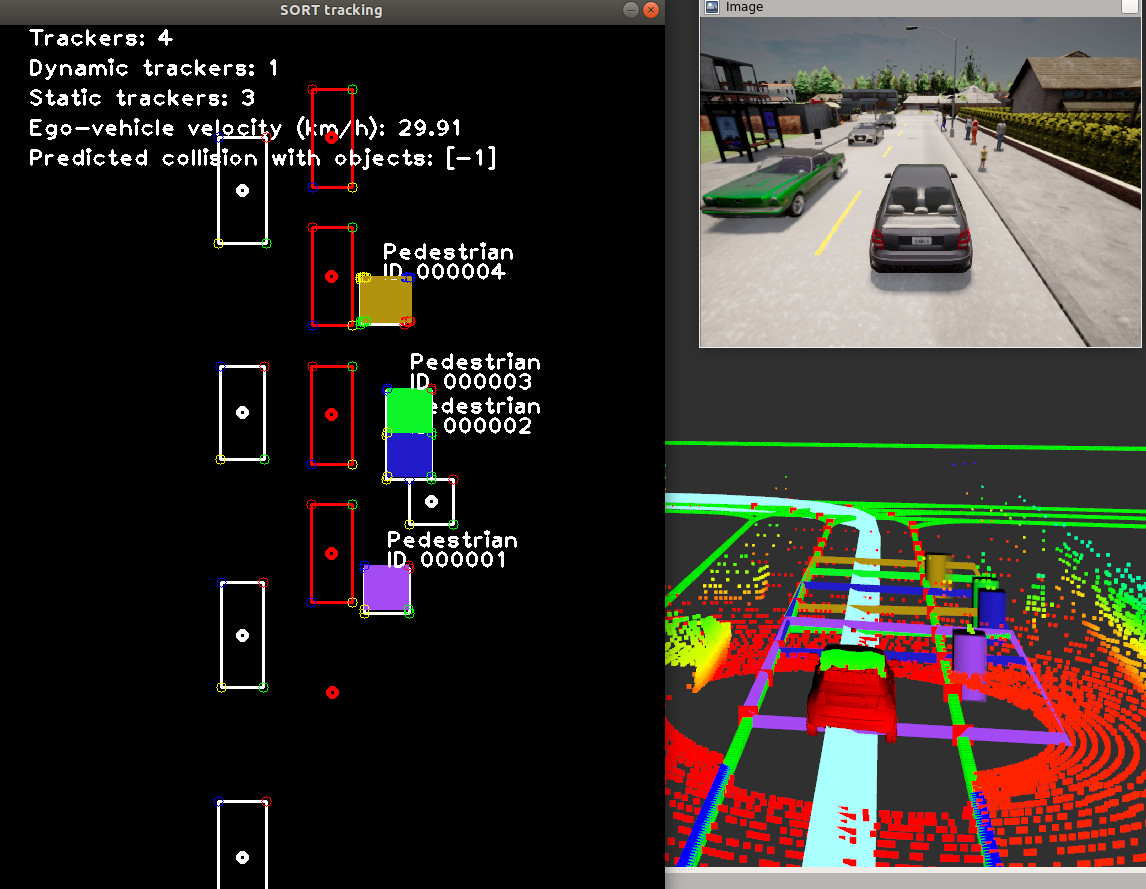
\includegraphics[width=0.8\textwidth]{4_filtering_process_example.jpg}
	\caption{Vulnerable Road Users (VRUs) are considered on the sidewalk if the they are close enough to the closest segment of the corresponding centerline.}
	\label{fig:4_filtering_process_example}
\end{figure} 

\section{Exploring Attention GAN for Vehicle Motion Prediction}
\label{sec:4_gan_lstm}

Despite the fact that SmartMOT illustrates a simple-yet-powerful tracking and prediction pipeline, traditional methods for \ac{MP} in the field of \ac{AD} are based on physical kinematic constraints and road map information with handcrafted rules. Though these approaches are sufficient in many simple situations (\ie vehicles moving in constant velocity or straightforward intersections), they fail to capture the rich behavior strategies and interaction in complex scenarios, in such a way they are only suitable for simple prediction scenes and short-time prediction tasks \cite{huang2022survey}. In that sense, as commented in Chapter \ref{sec:2_dl_based_mp}, recently \ac{DL} based methods have dominated this task and they usually follow an encoder-decoder paradigm. 

Prior knowledge on \ac{MP} in pedestrian datasets like ETH \cite{pellegrini2009you} or UCY \cite{lerner2007ucydata} usually focuses on deep methods such as \acp{LSTM} \cite{hochreiter1997long} and \acp{GAN} \cite{goodfellow2020generative}. SocialLSTM \cite{alahi2016social} proposes an \ac{LSTM}-based model that can jointly predict the paths of all agents in the scene taking into account the common sense rules and social conventions using a social-pooling module. SocialGAN \cite{gupta2018social} enhances SocialLSTM with a generative adversarial framework, introducing a variety loss that encourage the network to cover the space of plausible paths and proposing a novel pooling global social pooling vector that encodes the subtle cues for all agents involved in the scene. SoPhie \cite{sadeghian2019sophie} considers not only the path history of all agents but also the physical context information (captured by a top-view static image, computing salient regions of the scene), combining physical and social attention mechanisms in order to help the model knows what to extract and where to focus. Goal-GAN \cite{dendorfer2020goal} predicts the most likely goal points of the agent of interesting, estimating a set of trajectories towards these potential future candidates using both physical and social context, as proposed by \cite{sadeghian2019sophie}. On the other hand, in the context of vehicle prediction \cite{chang2019argoverse, caesar2020nuscenes}, prior information takes more importance regarding the risk at certain velocities in urban / highway environments in order to perform safe navigation.

As stated in Chapter \ref{sec:2_dl_based_mp}, HD maps have been widely adopted to provide a preliminary raw physical context and then apply data-driven approaches. Recent learning-based approaches \cite{hong2019rules, casas2018intentnet}, which present the benefit of having probabilistic interpretations of different behaviour hypotheses, require to build a representation to encode the trajectory and map information. \cite{hong2019rules} assumes that detections around the vehicle are provided and focuses its work on behaviour prediction by encoding entity interactions with ConvNets. Intentnet \cite{casas2018intentnet} proposes to jointly detect traffic participants (mostly focused on vehicles) and predict their trajectories using raw LiDAR pointcloud and rendered HD map information. PRECOG \cite{rhinehart2019precog} aims to capture the future stochasiticity by flow-based generative models. Furthermore, MultiPath \cite{chai2019multipath} uses ConvNets as encoder and adopts pre-defined trajectory anchors to regress multiple possible future trajectories. 

\subsection{Social Attention}
\label{subsec:4_gan_lstm_social_attention}

In a similar way to humans that pay more attention to close obstacles, people walking towards them or upcoming turns rather than considering the presence of people or building far away, the perception layer of a self-driving car must be modelled to focus more on the more relevant features of the scene. Social Attention is a mechanism that allows selective interactions within relevant agents. SoPhie \cite{sadeghian2019sophie} computes a different context vector for each agent, in such a way other agents features are sorted in terms of their relative distance to the agent of interest. Then, a soft attention mechanism is used to compute a context feature vector, which represents the social context. Nevertheless, a fixed size ($N_{\text{max}}$ agents) list that considers the context of all agents is sensitive to small variations \cite{mercat2020multi} of other agents positions. In that sense, SocialWays \cite{amirian2019social} presents a hand-crafted relative geometric feature to produce a set of normalized weights, in such a way the context vector represents a convex sum of other feature vectors (context of each agent) that is invariant to the ordering. 

However, these attention mechanisms were not designed to model complex interactions, no more than angles and distances due to the inherent problem of pedestrian prediction, in such a way we must find this challenging interactions in the vehicle motion prediction task to account for specific behaviours like overtaking, Adaptive Cruise Control (ACC), emergency braking or yielding. GRIP \cite{li2019grip} proposes a graph representation of vehicle neighbours, taking into account local interactions among vehicles withing a \textit{d} distance threshold around the target agent. 

\cite{vemula2018social} use a dot product attention module (inspired from the attention mechanism proposed by \cite{vaswani2017attention} for sentence translation), allowing joint forecast of every agent in the scene without spatial limitations, considering long range interactions regardless the ordering of the input vehicles tracks and the number of vehicles. Moreover, \cite{vemula2018social} combines this dot product with a spatio-temporal graph representation to take into account temporal and spatial dependencies of the agents, such as their absolute/relative positions and time step movements. \cite{mercat2020multi} present a multi-head extension of this dot attention mechanism, where each agent is embedded by means LSTMs before computing the dot product attention in order to produce social interactions. 

\subsection{Our GAN approach}
\label{subsec:4_gan_lstm_ours}

In this work, we aim to develop a model \cite{gomez2022exploring} that can successfully predict plausible future trajectories in the context of vehicle prediction, taking into account not only the past trajectory of the corresponding agent but also the past state of the most relevant obstacles around it and HD map information to compute a set of acceptable target points representing the physical constraints for our problem.

When vehicles drive through a traffic scenario, they usually aim to reach partial goals, depending on their predefined navigation route and scene context (both physical and social), until they finally arrive at their final destination. Formally, given a certain goal, vehicles must face different traffic rules and other agents along their way to reach their final destination. Regarding this, our model takes computes both the social context and acceptable target points for the corresponding agent given its past trajectory and then generates plausible trajectories towards the estimated goals. As illustrated in Figure \ref{fig:4_ITSC_2022}, our model consists of three main blocks:

\begin{itemize}
	\item \textit{Target Points Extractor}: Combines HDMap information and dynamic features of the target agent (speed and orientation) to generate acceptable target points in the driveable area.
	\item \textit{Attention module}: Computes the agent's dynamic features recursively by means a LSTM unit and uses a Multi-Head Self Attention module to capture complex social interactions among agents.
	\item \textit{GAN module}: Given the target points and highlighted social features, this module generates plausible and realistic trajectories using a LSTM based decoder, which represents the generator. Discriminator is applied to enhance the performance of the generator by forcing it to compute more realistic predictions.
\end{itemize} 

\begin{figure}[h] 
	\centering
	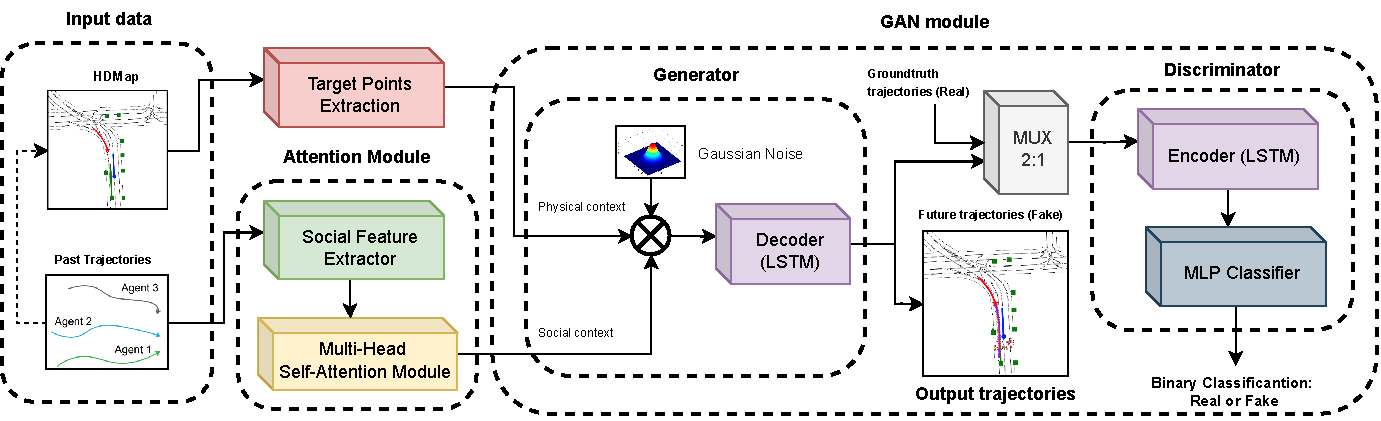
\includegraphics[width=\textwidth]{4_ITSC_2022.pdf}
	\caption[Overview of our Attention-based Generative Model]{Overview of our \textbf{Attention-based Generative Model}. We distinguish three main blocks: 1) \textbf{Target points extractor}, which uses HDMap information and agent past trajectory to compute acceptable target points, 2) \textbf{Attention module}, responsible for encoding the trajectories of the surrounding vehicles and applying Multi-Head Self-Attention, 3) \textbf{LSTM based GAN module}, which consists of a LSTM based decoder as the ''generator", in charge of taking into account the estimated target locations and the dynamic feature to generate the future trajectories, and a discriminator to force the generator to produce more realistic predictions.}
	\label{fig:4_ITSC_2022}
\end{figure}

Figure \ref{fig:4_ITSC_2022} illustrates an overview of our model. Next, we describe the different blocks of our model.

\subsubsection{Target points extraction}
\label{subsubsec:4_gan_lstm_target_points_extraction}

Multiple approaches have tried to predict realistic trajectories by means of learning physically feasible areas as heatmaps or probability distributions of the agent future location \cite{dendorfer2020goal, sadeghian2019sophie, gilles2021home}. These approaches require either a top-view RGB BEV image of the scene, or a HD Map with exhaustive topological, geometric and semantic information (commonly codified as channels). This information is usually encoded using a CNN and fed into the model together with the social agent information \cite{dendorfer2020goal, sadeghian2019sophie, gao2020vectornet}.

In our model, we propose we estimate the range of motion (360º) using a minimal HD Map representation that includes only the feasible area, where we can discretize the feasible area $\mathcal{F}$ (represented by a discrete grid of the \textit{width} x \textit{height} BEV map image where the pixels are driveable) as a subset of $r$ randomly sampled points $\{p_0 , p_1 ... p_r\}$ from such area in the map (easy to extract from a 1-channel binarized HD image) considering the orientation and velocity in the last observation frame for the agent. This step can be considered as pre-processing of the HD Map, therefore the model never sees the HD map image nor the whole graph of nodes. 

\begin{figure}[!ht]
	\centering
	\begin{subfigure}{0.24\textwidth}
		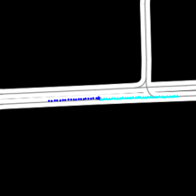
\includegraphics[width=\textwidth]{4_agent_trajectory.png}	
		\caption{(a)}
	\end{subfigure}
	\hfill
	\begin{subfigure}{0.24\textwidth}
		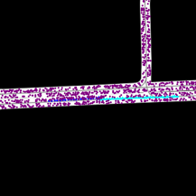
\includegraphics[width=\textwidth]{4_feasible_area_discretization.png}
		\caption{(b)}
	\end{subfigure}
	\hfill
	\begin{subfigure}{0.24\textwidth}
		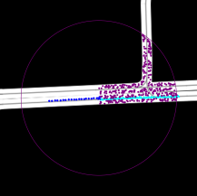
\includegraphics[width=\textwidth]{4_non_holonomic_filter.png}
		\caption{(c)}
	\end{subfigure}
	\hfill
	\begin{subfigure}{0.24\textwidth}
		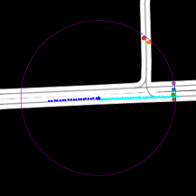
\includegraphics[width=\textwidth]{4_multimodal_clustering.png}
		\caption{(d)}
	\end{subfigure}
	\caption[Target Points Estimation from the Feasible area process]{Target Points Estimation from the Feasible area process: (a): Agent Past Trajectory (\textcolor{blue}{past observations} and \textcolor{aqua}{ground-truth}), (b) Feasible area discretization (random points in the driveable area), (c) Non-holonomic-based dynamic filter (both angle and velocity), (d) Multimodal clustering to get the final proposals}
	\label{fig:4_target_points_extraction}
\end{figure}

Figure \ref{fig:4_target_points_extraction} summarizes step-by-step the whole process. First, we calculate the driveable area (white area in Figure \ref{fig:4_target_points_extraction}) around the vehicle considering a hand-defined \textit{d} threshold.

Then, we consider the dynamic features of the agent of interest in the last observation frame $t_{obs}$ to compute acceptable target points in local coordinates. As we will detail in future sections, the Argoverse 1 Motion Forecasting dataset focuses on estimating the future prediction of a particular target agent. On top of that, the aforementioned dynamic features (orientation and velocity) are not provided, in such a way they must be calculated. Since the trajectory data are noisy with tracking errors, as expected from a real-world dataset, simply interpolating the coordinates between consecutive time steps, assuming constant frequency, results in noisy estimation. Then, in order to estimate the orientation and velocity of the target agent in the last observation frame $t_{obs}$, we compute a vector for each feature given:

\begin{equation}
	\begin{split}
		\theta_{i}=\arctan{(\frac{y_{i}-y_{i-1}}{x_{i}-x_{i-1}})} \\
		v_{i}=\frac{X_{i}-X_{i-1}}{t_{i}-t_{i-1}} 
	\end{split}
\end{equation}
 
where $X_{i}$ represents the 2D position of the agent at each observed frame $i$ as state above. Once both vectors are computed, we obtain a smooth estimation as proposed by \cite{tang2021exploring} of the heading angle (orientation) and velocity by assigning less importance (higher forgetting factor) to the first observations, in such a way immediate observations are the key states to determine the current spatio-temporal variables of the agent, as depicted in Equation \ref{eq:4_dynamic_feats_last_observation_frame}, which applies to both the orientation and velocity vector: 

\begin{equation}
	\hat{\psi}_{T_h} = \sum_{t=0}^{T_h}\lambda^{T_h - t}\psi_t
	\label{eq:4_dynamic_feats_last_observation_frame}
\end{equation}

where $T_h$ is the number of observed frames, $\psi_t$ is the estimated orientation/velocity at the $t_{i}$ frame, $\lambda\in(0, 1)$ is the forgetting factor, and $\hat{\psi}_{t_obs}$ is the smoothed orientation/velocity estimation at the last observed frame. After estimating these variables, we calculate the range of motion around the target agent as a circle with radius: $H * \psi_{v}$ where $\psi_{v}$ is the estimated velocity using Equation \ref{eq:4_dynamic_feats_last_observation_frame} and $H=3$ is the time-horizon of 3s. After that, we randomly sample $r$ points $p \in \mathcal{F}$ in this range considering a constant velocity model during the prediction horizon and the estimated orientation, assuming non-holonomic constraints \cite{triggs1993motion} which are inherent of standard road vehicles, that is, the car has three degrees of freedom, its position in two axes and its orientation, and must follow a smooth trajectory in a short-mid term prediction. Finally, we estimate $k$ target points (one per mode required in the future prediction) by means of the k-means \cite{ahmed2020k} clustering algorithm. This clustering method, originally from signal processing, that aims to partition n observations into k clusters in which each observation belongs to the cluster with the nearest mean (cluster centers or cluster centroid), serving as a prototype of the cluster. In this particular model, we focus on unimodal prediction, that is, the model must reason the most plausible future trajectory based on the agents past observations, attention-based social interaction and target points as physical context.

This representation not only reunites information about the feasible area around the agent, but also represents potential \textbf{Target points} \cite{dendorfer2020goal} (\ie potential destinations or end-of-trajectory points for the agents). Moreover, this information is \textit{"cheap"} and \textit{interpretable}, therefore, we do not need further exhaustive annotations from the HD Map in comparison with other methods like HOME, which gets as input a 45-channel encoded map~\cite{gilles2021home}.
%
We concatenate this information, as 2D vector $\mathcal{V}$, together with the model social context features to generate more realistic trajectories (see Figure \ref{fig:4_ITSC_2022}).

\subsubsection{Attention module}

Our model takes as social input the past $n$ observations in map (global) coordinates for each agent in the scene, encoding these trajectories as a preliminary stage before feeding a Multi-Head Self-Attention (MHSA) \cite{vaswani2017attention} module that computes the social context of the scene, as observed in Fig. \ref{fig:4_ITSC_2022}. The past trajectory of an agent is transformed to relative (local coordinates) displacement vectors $\left( \Delta x_i^t, \Delta y_i^t \right)$ and embedded into a higher dimensional vector with a Multi-Layer Perceptron (MLP), which serves as input of the LSTM unit, dynamic feature extractor to capture the speed and direction of the corresponding agent. Then, the hidden state of the LSTM ($h_{M\!E}$) is used by the MHSA module that learns complex social interactions while being invariant to their number and ordering, avoiding a fixed size ($N_{\text{max}}$ agents) list which would be sensitive to small variants in the agent's positions. In this context, each agent of the scene should pay attention to specific features from the most relevant agents around it. The Multi-Head Self-Attention module consists of several heads that given the encoded trajectories produces feature vectors that encode all pairwise relations among agent's information. Implementation details are specified in Chapter \ref{sec:5_motion_prediction_datasets}.

\subsubsection{GAN module}

To capture the stochastic nature of motion prediction, state-of-the-art methods leverage the power of generative models, such as Variational Autoencoders (VAEs) and Generative Adversarial Networks (GANs). In our work we use an adversarial framework in order to train our trajectory generator, responsible for generating physically and realistic feasible trajectories. In a GAN, the Generator (which after being trained will be the inference network) and Discriminator networks compete in a two-player min-max game \cite{goodfellow2020generative}, as observed in Equation \ref{eq:4_min_max_game}. While the generator aims at producing feasible trajectories, the discriminator learns to differentiate between fake and real samples, in other words, ground-truth (which are feasible by definition) and inferred trajectories, in such a way the tasks of the discriminator is to enhance the performance of the generator by forcing it to compute more realistic predictions, more and more similar to the ground-truth trajectory. As a result, the generator should be able to produce outputs which the discriminator cannot discriminate clearly, indicating that the output is realistic. 

\begin{eqnarray}
	\label{eq:4_min_max_game}
	&&\hspace{-10mm} \min_{Gen} \max_{Dis} V(Dis, Gen)=E_{X \sim p_{data}(X)}[\mbox{log} Dis(X,Y)] \nonumber \\
	&&\hspace{15mm} + E_{z \sim p_z(z)}[\mbox{log} (1 - Dis(X, Gen(X,z)))],
\end{eqnarray}

In the present case, the generator, also identified as the routing module, is represented by a decoder LSTM  ($LSTM_{gen}$) and the discriminator by a classifier LSTM ($LSTM_{dis}$) so as to estimate the temporally dependent future states. Similar to the conditional GAN proposed by \cite{sadeghian2019sophie}, the input to our generator is a concatenation of a white noise vector $z$ sampled from a multivariate normal distribution, being the physical context (goal points in relative coordinates in the last observation frame, $C_{Ph(i)}^{t_{obs}}$) and social context (interactions among agents, $C_{So(i)}^{1:t_{obs}}$) its conditions. Then, the generated future trajectory for a particular agent is modelled as Eq. \ref{eq:4_gen_dec}:

\begin{eqnarray}
	\label{eq:4_gen_dec}
	& \hat{Y}_i^{t_{obs}:t_{pred}} = LSTM_{gen}\big(C_{Ph(i)}^{t_{obs}}; C_{So(i)}^{1:t_{obs}}; z\big)
\end{eqnarray}

On the other hand, the input of the discriminator is a randomly chosen trajectory sample from the either predicted future trajectory or ground-truth for the corresponding agent up to $t = t_{obs} + t_{pred}$ frame, i.e.  $T_i^{t_{obs}:t_{pred}}\sim p(\hat{Y}_i^{t_{obs}:t_{pred}},Y_i^{t_{obs}:t_{pred}})$.

\begin{eqnarray}
	\label{eq:4_dis}
	\hat{L}_{i}^{t_{obs}:t_{pred}} = LSTM_{dis}(T_i^{t_{obs}:t_{pred}})
\end{eqnarray}

Then, the discriminator returns a label $\hat{L}_{i}^{t_{obs}:t_{pred}}$ for the chosen trajectory indicating whether the trajectory is ground-truth (real) $Y_i^{t_{obs}:t_{pred}}$ or predicted (fake) $\hat{Y}_i^{t_{obs}:t_{pred}}$, being the labels 0 and 1 for fake and real trajectories respectively. Equation \ref{eq:4_dis} summarizes the discriminator working principles. 

\subsubsection{Losses}

To train our \ac{GAN} model, we use the following losses:

\begin{eqnarray}
	\label{eq:obj}
	W^* =\operatorname*{argmin}_W \quad\mathbb{E}_{i,\tau}[\lambda_{gan} \mathcal{L}_{GAN}\big(\hat{L}_{i}^{t_{obs}:t_{pred}}, L_{i}^{t_{obs}:t_{pred}} \big)+ \nonumber\\
	\lambda_{ade} \mathcal{L}_{L2}(\hat{Y}_i^{t_{obs}:t_{pred}},Y_i^{t_{obs}:t_{pred}})+ \nonumber\\
	\lambda_{fde} \mathcal{L}_{L2}(\hat{Y}_i^{t_{obs}+t_{pred}},Y_i^{t_{obs}+t_{pred}})],
\end{eqnarray}
%
where $W$ is the collection of the weights of all networks used in our model and the different $\lambda$ represent the corresponding regularizers between these losses. As stated in Eq. \ref{eq:4_min_max_game}, $\mathcal{L}_{GAN}$ represents the min-max game where the generator tries to minimize the function while the discriminator tries to maximize it. ADE loss function is commonly used to compute the average error between the predicted trajectories and the corresponding ground-truth. Moreover, we add FDE loss function to explicitly optimize the distribution towards the final real point.

\section{Efficient Baselines for Motion Prediction in Autonomous Driving}
\label{sec:4_efficient_baselines}

As observed in the previous section, our \ac{GAN}-based model (more specifically the generator) was able to compute the deep context regarding the agents past observations, attention-based social interaction and target points as physical context, but the prediction was limited to the unimodal case. In other words, the \ac{GAN}-based model is able to reason more complex interactions and future behaviours than SmartMOT (physics-based prediction), but it lacks one of the main features of a deep learning-based model as a preliminary stage before the local planning or decision-making layers: Multimodality. On top of that, at this point of the thesis the literature was re-visited and despite \acp{GAN}-based approaches \cite{sadeghian2019sophie, dendorfer2020goal, gupta2018social, gomez2022exploring} provide certain control since they are focused on more simple methods framed in an adversarial training, most competitive approaches on \ac{MP} benchmarks in the field of \ac{AD}, such as Argoverse \cite{chang2019argoverse}, NuScenes \cite{caesar2020nuscenes} or Waymo \cite{ettinger2021large}, \textbf{do not} use adversarial training, where the training complexity is one the main reasons.

In that sense, considering the trade-off between curated input data and complexity, we aim to achieve competitive performance in the \ac{MP} using powerful DL techniques in terms of prediction metrics (\ac{minADE}, \ac{minFDE}), including attention mechanisms and \acp{GNN}, while reducing the number of parameters of operations with respect to other \ac{SOTA} methods. In particular, we propose two baselines, social and map baseline. 

The only inputs for the social baseline are the agent past trajectories and their corresponding interactions. On the other hand, for the map baseline, we propose an extension with respect to our previous target points proposals where, based on a simple-yet-powerful map pre-processing algorithm where the corresponding agent trajectory is initially filtered, the feasible area with which the agent can interact is computed. In spite the fact that topological, semantic and geometric information are involved while computing this area due to road connectivity, we only retrieve the geometric information of the feasible area proposals in an efficient and elegant way. Therefore, our models do not require full-annotated (including, topological, geometric and semantic) HD Map information as input or even rasterized \ac{BEV} representations of the scene to compute the physical context. Figure \ref{fig:4_TITS_2023} illustrates an overview of our final approach.

\begin{figure*}[!ht]
	\centering
	\setlength{\tabcolsep}{2.0pt}
	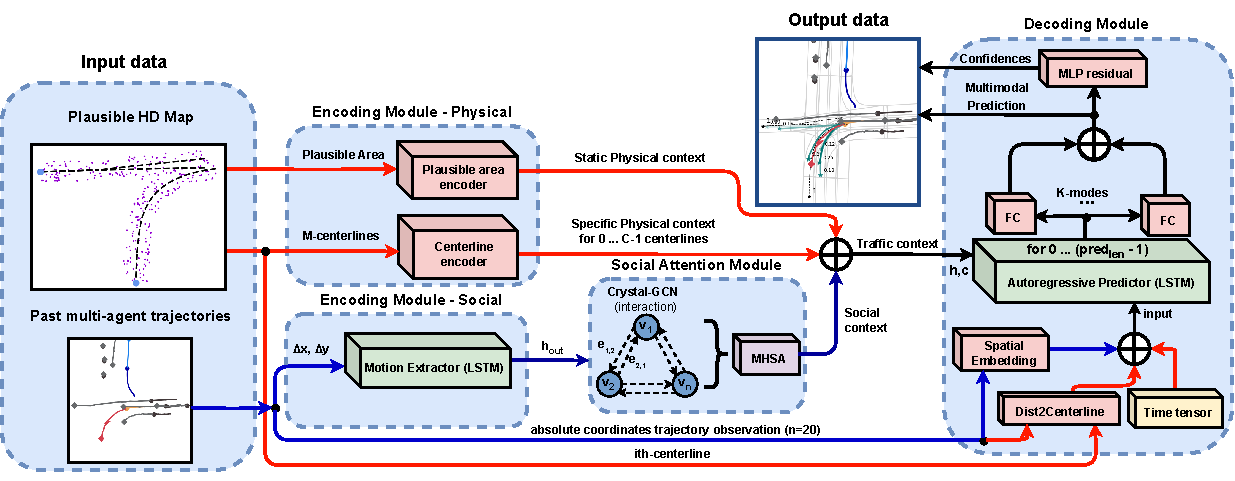
\includegraphics[width=0.95\linewidth]{4_TITS_2023.pdf}
	\caption[Overview of our final efficient baseline model]{Overview of our final efficient baseline model (\textbf{\textcolor{blue}{Blue links}} and \textbf{\textcolor{red}{Red links}} represent \textbf{\textcolor{blue}{Social}} and \textbf{\textcolor{red}{Map}} information respectively). We distinguish three main blocks: 1) \textbf{Encoding module}, which uses plausible HD Map information (specific centerlines and driveable area around) and agents past trajectories to compute the motion and physical latent features, 2) \textbf{Social Attention module}, which calculates the interaction among the different agents and returns the most relevant social features, 3) \textbf{Decoding module}, responsible for calculating the multimodal prediction by means of an auto-regressive strategy concatenating low-level map features and social features as a baseline, as well as iterating over the different latent centerlines for specific physical information per mode.}
	\label{fig:4_TITS_2023}
\end{figure*}

\subsection{Social Baseline}
\label{subsec:4_efficient_baselines_social}

Our social baseline is inspired in the architecture proposed by \cite{schmidt2022crat}. It uses as input the past trajectories of the most relevant obstacles as relative displacements to feed the Encoding Module (Figure \ref{fig:4_TITS_2023}). Then, the social information is computed using a \ac{GNN}, in particular Crystal-Graph Convolutional Network (\textbf{Crystal-GCN}) layers \cite{xie2018crystal, schmidt2022crat}, and Multi-Head Self Attention (MHSA) \cite{vaswani2017attention} to obtain the most relevant agent-agent interactions. Finally, we decode this latent information using an \textbf{autoregressive} strategy where the output at the \textit{i-th} step depends on the previous one for each mode respectively in the Decoding Module. The following sections provide in-depth description of the aforementioned modules.

\subsubsection{Preprocessing of past trajectories}
\label{subsubsec:4_efficient_baselines_social_preprocessing}

Multiple methods \cite{liang2020learning, schmidt2022crat} consider only the vehicles that are observable at \textit{t=0}, handling those agents that are not observed over the full sequence spectrum (observation length = \textit{$obs_{len}$} + prediction length = \textit{$pred_{len}$}) by concatenating a binary flag $b_i^t$ that indicates if the agent is padded or not. In our case, we consider the agents that have information over the full history horizon $T_h$ = \textit{$obs_{len}$} + \textit{$pred_{len}$} (\emph{e.g.} 5s timeframe for Argoverse), reducing the number of agents to be considered in complex traffic scenarios. Furthermore, to make the model translation and rotation invariant, the coordinate system in our model is \ac{BEV} centered of a given target agent at $t = 0$, and we use the orientation from the target location given in the same timestamp as the positive $x$-axis. Note that this representation will benefit the model to have a common representation to enhance the generalization of the model and prevent overfitting. Once the scene has been translated and rotated, instead of using absolute 2D-BEV (\textit{xy} plane), the input for the agent \textit{i} is a series of relative displacements:

\begin{equation}
	\Delta \boldsymbol{\nu}^{t}_i = \boldsymbol{\nu}^{t}_i - \boldsymbol{\nu}^{t-1}_i
\end{equation}

Where $\boldsymbol{\nu}^{t}_i$ represents the state vector (in this case, \textit{xy} position of the agent \textit{i} at timestamp \textit{t}.

\subsubsection{Encoding of past trajectories}
\label{subsubsec:4_efficient_baselines_social_encoding}

Unlike other methods, we do not limit nor fix the number of agents per sequence. Given the relative displacements of all different agents, a single \ac{LSTM} is used to compute the temporal information of each agent in the sequence:

\begin{equation}
	out, \mathbf{h_{out}}, \mathbf{c_{out}} = \mathrm{LSTM}(\Delta \boldsymbol{\nu}^{obs_{len}}, \mathbf{h_{in}}, \mathbf{c_{in}})
\end{equation}

This LSTM encoder shares the weights for all vehicles in the batch. The input hidden and cell vectors ($\mathbf{h_{in}}, \mathbf{c_{in}}$) are initialized with a tensor of zeros. $\Delta \boldsymbol{\nu}^{obs_{len}}$ represents the relative displacements over the whole past horizon $obs_{len}$. In order to feed the agent-agent interaction module (Social Attention Module in Figure \ref{fig:4_TITS_2023}), we take the output hidden vector ($\mathbf{h_{out}}$).

\subsubsection{Social Attention module}
\label{subsubsec:4_efficient_baselines_social_interactions}

After encoding the past history of each vehicle in the sequence, we compute the agent-agent interactions to obtain the most relevant social information of the scene. For this purpose, we construct an interaction graph using Crystal-GCN \cite{xie2018crystal} \cite{schmidt2022crat}. , originally developed for the prediction of material properties, allowing to efficiently leverage edge features. Then, \ac{MHSA} \cite{vaswani2017attention} is applied to enhance the learning of agent-agent interactions. 

Before creating the \textbf{interaction mechanism}, we split the temporal information in the corresponding scenes, taking into account that each traffic scenario may have a different number of agents. The interaction mechanism is defined in \cite{schmidt2022crat} as a bidirectional fully-connected graph, where the initial node features $\mathbf{v}_i^{(0)}$ are represented by the latent temporal information for each vehicle $\mathbf{h}_{i,out}$ computed by the motion history encoder. On the other hand, the edges from node \textit{k} to node \textit{l} is represented as the vector distance ($\mathbf{e}_{k,l}$) between the corresponding agents at t = \textit{$obs_{len}$} in absolute coordinates, where the origin of the sequence ($x=0,y=0$) is represented by the position of the target at t = \textit{$obs_{len}$}:

\begin{equation}
	\mathbf{e}_{k,l} = \boldsymbol{\nu}^{obs_{len}}_k - \boldsymbol{\nu}^{obs_{len}}_l \text{,}
\end{equation}

Given the interaction graph (nodes and edges), the Crystal-GCN, proposed by \cite{xie2018crystal}, is defined as:

\begin{multline}
	\mathbf{v}_i^{(g+1)} = \mathbf{v}_i^{(g)} + \\
	\sum_{j = 0 \textbf{:} j \neq i }^{N} \sigma \left( \mathbf{z}_{i,j}^{(g)} \mathbf{W}_\mathrm{f}^{(g)} + \mathbf{b}_\mathrm{f}^{(g)} \right)
	\odot \mu \left( \mathbf{z}_{i,j}^{(g)} \mathbf{W}_\mathrm{s}^{(g)} + \mathbf{b}_\mathrm{s}^{(g)}  \right) \text{.}
\end{multline}

This operator, in contrast to many other graph convolution operators \cite{zeng2021lanercnn} \cite{liang2020learning}, allows the incorporation of edge features in order to update the node features based on the distance among vehicles (the closer a vehicle is, the more is going to affect to a particular node). As stated by \cite{schmidt2022crat}, we use $L_g = 2$ layers of the GNN ($g \in 0, \dots , L_g$ denotes the corresponding Crystal-GCN layer) with ReLU and batch normalization as non-linearities between the layers. $\sigma$ and $\mu$ are the sigmoid and softplus activation functions respectively. 

Moreover, $\mathbf{z}_{i,j}^{(g)} = ( \mathbf{v}_i^{(g)} || \mathbf{v}_j^{(g)} ||\mathbf{e}_{i,j} )$ corresponds to the concatenation of two node features in the \textit{$g_{th}$} GNN layer and the corresponding edge feature (distance between agents), N represents the total number of agents in the scene and $\mathbf{W}$ and $\mathbf{b}$ the weights and bias of the corresponding layers respectively.

After the interaction graph, each updated node feature $\mathbf{v}_i^{(L_g)}$ contains information about the temporal and social context of the agent \textit{i}. Nevertheless, depending on their current position and past trajectory, an agent may require to pay attention to specific social information. To model this, we make use of a scaled dot-product Multi-Head Self-Attention mechanism \cite{vaswani2017attention} which is applied to the updated node feature matrix $\mathbf{V}^{(L_g)}$ that contains the node features $\mathbf{v}_i^{(L_g)}$ as rows. 

Each head $h \in 1,\dots, L_h$ in the MHSA mechanism is defined as:

\begin{equation}
	\mathrm{head}_h = \mathrm{softmax} \left( \frac{\mathbf{V}^{(L_g)}_{Q_h} \mathbf{V}^{(L_g) T}_{K_h}}{\sqrt{d}}  \right) \mathbf{V}^{(L_g)}_{V_h} \text{.}
\end{equation}

where $\mathbf{V}^{(L_g)}_{Q_h}$ (Query), $\mathbf{V}^{(L_g)}_{K_h}$ (Key) and $\mathbf{V}^{(L_g)}_{V_h}$ (Value) represent the \textit{$h_{th}$} head linear projections of the node feature matrix $\mathbf{V}^{(L_g)}$ and $d$ is the normalization factor corresponding to the embedding size of each head. For our purpose, we use $L_h = 4$ as the total number of heads. 

The result of the softmax weights multiplied by the node feature matrix $\mathbf{V}^{(L_g)}_{V_h}$ (Value) is often referred as the attention weight matrix, representing in this particular case pairwise dependencies among vehicles.

Finally, the updated node feature matrix $\mathbf{SATT}$ is computed as the combination of the different attention heads in a single matrix:

\begin{equation}
	\mathbf{SATT} = (\mathrm{head}_1 || \dots || \mathrm{head}_{L_h}) \mathbf{W}_\mathrm{o} + 
	\begin{pmatrix}
		\mathbf{b}_\mathrm{o}\\
		\vdots \\
		\mathbf{b}_\mathrm{o}
	\end{pmatrix}.
\end{equation}

Where each row of the final social attention matrix $\mathbf{SATT}$ (output of the social attention module, after the GNN and MHSA mechanisms) represents the interaction-aware feature of the agent \textit{i} with surroundings agents, considering the temporal information under the hood, being $\mathbf{W}_\mathrm{o}$ / $\mathbf{b}_\mathrm{o}$ the corresponding weight and bias of the layer that merges the different attention heads. As we will see in Chapter \ref{sec:5_motion_prediction_datasets}, regarding the Argoverse 1 Motion Forecasting benchmark, we \textbf{only consider} the row of the final matrix that takes into account the interactions of the target agent with surrounding obstacles.

\subsection{Map Baseline} 
\label{subsubsec:4_efficient_baselines_map_baseline}

As mentioned before, in this work we extend our social baseline using minimal HD map information, from which we discretize the feasible area $\mathcal{P}$ of the target agent as a subset of $r$ randomly sampled points $\{p_0 , p_1 ... p_r\}$ (low-level features) around the plausible centerlines (high-level and well-structured features) considering the velocity and acceleration of the corresponding agent in the last observation frame, as observed in Figure \ref{fig:4_efficient_baselines_hdmap_filtering}. As stated in Section \ref{subsec:4_gan_lstm_ours}, this is a map preprocessing step, therefore the model never sees the HD map (either vectorized or rasterized) image nor the whole graph of nodes.

\subsubsection{Centerlines proposals and Feasible area points} 
\label{subsubsec:4_efficient_baselines_preprocessing_map}

In a similar way to the target points computed in our \ac{GAN}-based model, we want to compute the heuristic proposals for each agent. Nevertheless, instead of limiting the map baseline to some discrete target points, now we aim to compute the most plausible future centerlines (that is, the center of the lane) as a connection of nodes (waypoints). Considering lane connectivity, multiple approaches have tried to predict realistic trajectories by means of learning physically feasible areas as heatmaps or probability distributions of the agent’s future location~\cite{dendorfer2020goal, sadeghian2019sophie, gilles2021home}. \cite{liang2020learning} represents the map as a set of lanes and their connectivity (predecessor, successor, right neighbour, left neighbour), taking into account all lanes whose distance from the target agent is smaller than 100 m as the input, regardless the orientation or the velocity of the vehicle. On the other hand, \cite{djuric2021multixnet} encodes static elements such as crosswalks, lane, road boundaries and intersections that are included in a local map 150m x 100m centered in the corresponding vehicle  as a multi-channel image.  These approaches require either a top-view RGB \ac{BEV} image of the scene, or a HD map with exhaustive topological, geometric and semantic information (commonly codified as channels). This information is usually encoded using a \ac{CNN} and fed into the model together with the social agent's information \cite{dendorfer2020goal, sadeghian2019sophie, gao2020vectornet}. 

As observed, when trying to utilize HD map information, specially in terms of lane proposals, most SOTA methods utilize this physical to enhance the latent information to decode the future trajectories, but heavy computation or raw data features are required. 

\begin{figure*}[]
	\centering
	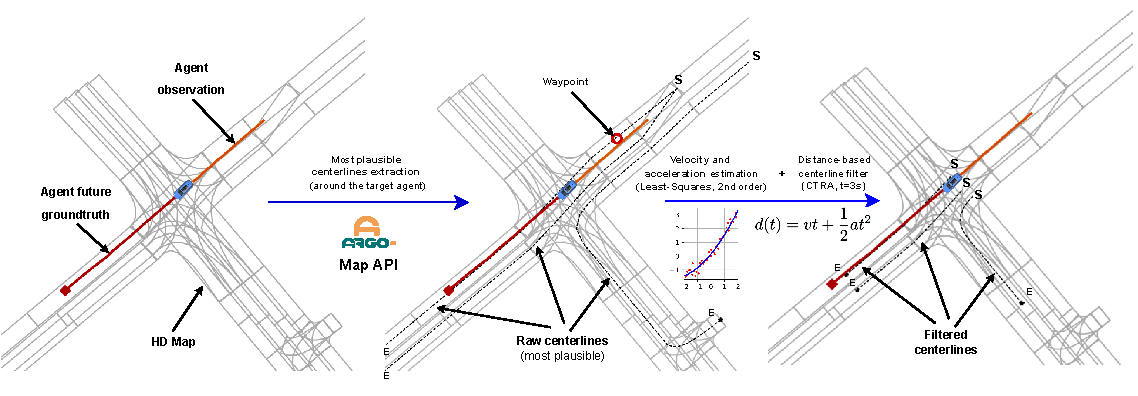
\includegraphics[width=0.95\linewidth]{4_compute_centerlines_argo_1.pdf}
	
	\caption{Plausible centerlines estimation. Left: General view of the scene, only considering the target agent (\textbf{\textcolor{YellowOrange}{observation (2 s)}} and \textbf{\textcolor{red}{future ground-truth (3 s)}}) and HD Map around its last observation (position of the \textbf{\textcolor{blue}{blue}} vehicle). Center: \textbf{Centerlines} proposed by the Argoverse Map API (maximum number of centerlines M set to 3). Right: We filter the input observation by means of Least-Squares (2nd order) algorithm to estimate the velocity and acceleration of the agent. Then, the distance considering a CTRA (Constant Turn Rate Acceleration) model and a prediction horizon of 3 s are used computed to obtain the end-points \textbf{E} of the \textbf{final proposals}. Start-points \textbf{S} are the closest centerlines waypoints to the agent in the last observation frame.}
	\label{fig:4_efficient_baselines_hdmap_filtering}
\end{figure*}

\textbf{Effectively} and \textbf{efficiently} exploiting HD maps is a must for MP models to produce accurate and plausible trajectories in real-time applications, specially in the field of AD, providing specific map information to each agent based on its kinematic state and geometric HD map information. In that sense, we propose to obtain the most plausible \textit{M} lane candidates, we make use of the pertinent heuristic functions proposed by the Argoverse 1 Motion Forecasting dataset Map API \cite{chang2019argoverse} as illustrated by \cite{khandelwal2020if} to choose the closest centerlines to the last observation data of the target agent, which are going to represent its most representative future trajectories. On the other hand, as depicted in the \ac{MP} dataset used to train this model (Argoverse 1), vehicles are the only evaluated object category as the target agent. Then, considering a vehicle as a rigid structure with non-holonomic \cite{triggs1993motion} features (no abrupt motion changes between consecutive timestamps) and the road driving task is usually described as anisotropic \cite{ross1989planning} (most relevant features are found in a specific direction, in this case the lanes ahead). In other words, the agent should follow a smooth trajectory in a short-mid term prediction. The heuristic to obtain these centerlines is summarized as follows:

\begin{enumerate}
	\item Trajectory data presents noise associated to the real-world data capturing the exact position of the previously tracked vehices in real-world scenarios. Regarding this, we filter the agent trajectory as a polynomial curve fitting problem by means of the Least Squares ($2^{nd}$ order) per axis and Savitzky-Golais \cite{savitzky1964smoothing} algorithms to obtain a smooth representation of the position vector.
	
	\item By doing so, and assuming the agent is moving with a constant acceleration, we are able to calculate the subsequent derivatives (velocity and acceleration) of the target agent in $t_{obs_{len}}$. Then, a vector of $obs_{len}$ - 1 and $obs_{len}$ - 2 length is computed to estimate the velocity and acceleration respectively as $V_{i}=\frac{X_{i}-X_{i-1}}{t_{i}-t_{i-1}}$ and $A_{i}=\frac{V_{i}-V_{i-1}}{t_{i}-t_{i-1}}$, where $X_{i}={[x_{i},y_{i}]}$ represents the 2D position of the agent at each observed frame $i$.
	
	\item In order to compute the velocity, acceleration and yaw angle in the last observation frame, we compute a weighted mean by assigning less importance (weight) to the first positions of the corresponding vector and higher importance to the latter states, in such a way immediate past observations are the key states to determine the current spatio-temporal variables of the agent, as depicted in Equation \ref{eq:4_dynamic_feats_last_observation_frame}.
	
	\item We compute the future travelled distance by means of the well-known Constant Acceleration (CA) model:
	
	\begin{equation}
		d(t) = x_0 + vt + \frac{1}{2}at^2
	\end{equation}

	where $t$ corresponds to the prediction horizon $t_pred$, $x_0$ is equal to $0$ since we want to determine the travelled distance from the current position and $v$ and $a$ are the velocity and acceleration in the last observation frame previously calculated. Note that we assume that this is a \ac{CTRA} model, instead of only \ac{CA} in a specific direction, since the orientation is implicit in the lane boundaries. That's why it does not make sense to involve the orientation at frame $t=0$ in the travelled distance calculation.
	
	\item Get all lane candidates within a bubble, given the agent last observation and Manhattan distance.
	
	\item Expand the bubble until at least 1 lane is found.
	
	\item Once some preliminary proposals are found, we employ the Depth First Search (DFS) algorithm to get all successor and predecessor candidates, merging the past and future candidates and removing the overlapping ones.
	
	\item Then, we process these raw candidates so as to use them as plausible physical information. Given these raw lanes, we aim to limit the number of centerlines to a fixed number $M$. First, given the previously computed smoothed trajectory, we compute the closest centerlines to our current position since they will represent the most realistic future lanes in the traffic scenario. Second, we evaluate the above-mentioned travelled distance along the raw centerlines. We determine the end-point index $p$ of the centerline $m$ as the waypoint (each discrete node of the centerline) where the accumulated distance (considering the $\mathcal{L}_2$ distance between each waypoint) is greater or equal than the above-computed $d(obs_{len})$:
	
	\begin{equation}
		p \quad \textbf{:} \quad d(obs_{len}) \leq \sum_{p=start_{point}}^{centerline_{length}} \mathcal{L}_2(w(p+1),w(p))
	\end{equation}

	\item Finally, in order to have the same points (particularly, the number of points matches the prediction horizon $t_pred$, also referred as $pred_len$) per centerline, we interpolate them using a $1^{st}$ spline order, considering as start point the last agent observation and as end or goal point the aforementioned travelled distance along the corresponding centerline.
	
	\item Note that if the number of proposed centerlines is lower than a pre-defined number $M$, a virtual centerline is created and padded with zeros.
\end{enumerate}

Figure \ref{fig:4_efficient_baselines_hdmap_filtering} summarizes this HDMap filtering process, where we are able to estimate the preliminary centerlines proposals as a \textbf{simplified version of the HD map}. Moreover, Fig. \ref{fig:4_efficient_baselines_hdmap_filtered_examples} illustrates how after our filtering process the end-points of the plausible centerlines are noticeable closer to the ground-truth prediction at the final timestep. 

In addition to these \textbf{high-level} and well-structured centerlines, we apply point location perturbations to all plausible centerlines under a $\mathcal{N}(\mu, \sigma)$ [m] distribution~\cite{ye2021tpcn} in order to discretize the plausible area $\mathcal{P}$ as a subset of $r$ randomly sampled points $\{p_0 , p_1 ... p_r\}$ (\textbf{low-level} features) around the plausible centerlines. By doing this, we may have a common representation of the plausible area, defined as low-level map features. We make use of a normal distribution $\mathcal{N}$ to calculate these random points as an additional regularization term in a similar way that data augmentation is applied to the past trajectories. 

\begin{figure}[t!]
	\begin{subfigure}{0.5\textwidth}
		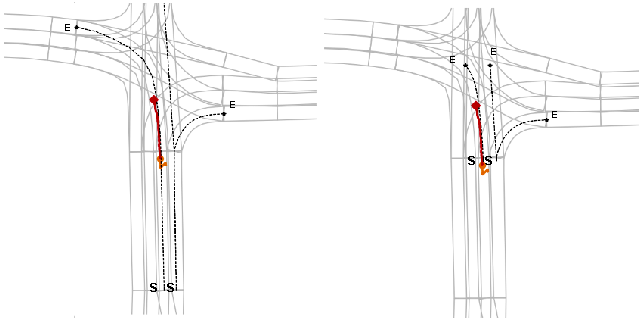
\includegraphics[width=\textwidth]{4_compute_centerlines_example_1.pdf}

	\end{subfigure}
	\hfill
	\begin{subfigure}{0.5\textwidth}
		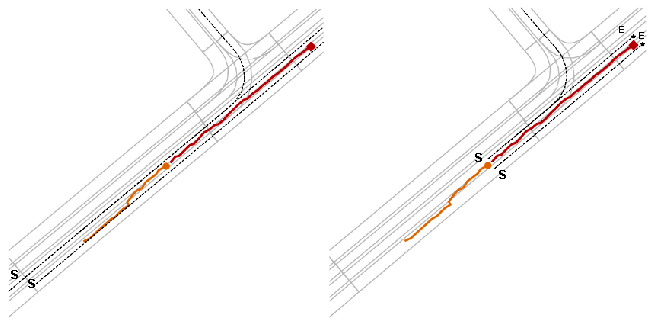
\includegraphics[width=\textwidth]{4_compute_centerlines_example_2.pdf}

	\end{subfigure}
	
	\caption{Some challenging examples of our preprocessing step to obtain relevant map features. In both scenarios the target agent (\textbf{\textcolor{YellowOrange}{observation (2 s)}} and \textbf{\textcolor{red}{future ground-truth (3 s)}}) presents a noticeable noisy past trajectory and the provided raw \textbf{centerlines} do not consider the current kinematic state of the vehicle. (a) The agent is stopped (maybe due to an stop, pedestrian crossing or red traffic light use case). We estimate a minimum travelled distance of 25 m in these situations to determine the centerline end-points \textbf{E}. (b) In this scenario, we can observe how the raw centerlines consider way more distance (both ahead and behind) than required. Our kinematic-based filter is able to minimize these proposals in an interpretable way to serve as prior information to the MP model
	}
	\label{fig:4_efficient_baselines_hdmap_filtered_examples}
\end{figure}

\subsubsection{Encoding module of map information}
\label{subsubsec:4_efficient_baselines_encoding_map}

In order to calculate the latent map information, we employ a plausible area and centerline encoder (Figure \ref{fig:4_TITS_2023}) to process the low-level and high-level map features respectively. Each of these encoders are represented by a Multi-Layer Perceptron (MLP). First, we flat the information along the points dimension, alternating the x-axis and y-axis information. Then, the corresponding MLP (three layers, with batch normalization, interspered ReLUs and dropout in the first layer) transforms the interpretable absolute coordinates around the origin ($x=0, y=0$) into representative latent physical information. The static physical context (output from the plausible area encoder) will serve as a common latent representation for the different modes, whilst the specific physical context will illustrate specific map information for each mode.

\subsection{Augmented Efficient baseline with Transformer Encoders}
\label{subsec:4_augmented_baseline}

Once the social and map baseline encoders are stated, we focus on a more powerful mechanism to encode the spatial and temporal information of inputs by encoding them into feature vectors. In that sense, we focus of designing an effective encoder transformer while keeping its structure as simple and efficient as possible. In a similar way to \cite{wang2023lane}, we adopt the combination of CNN/MLP, attention block and normalization, as observed in Figure \ref{fig:4_ITSC_2023}.

\begin{figure*}[!ht]
	\centering
	\setlength{\tabcolsep}{2.0pt}
	\includegraphics[width=0.95\linewidth]{4_ITSC_2023.pdf}
	\caption{Efficient baseline with transformer encoders to process the physical and social input}	
	\label{fig:4_ITSC_2023}
\end{figure*}

In order to encode the centerlines, we first use an MLP-based encoder to transform the input vector at each time stamp ($d_i^t$, which actually represents a plausible position of the target agent) into deep features:

\begin{equation}
	f_i^t=MLP_{\text{map}}\left(d_i^t ; W_{\text {map }}\right)
\end{equation}

where $MLP_{\text{map}}$ is a Multi-Layer (3) Perceptron with a ReLU asnon-linear layer and $W_{\text {map }}$ as the weight matrix that is learnable. However, to predict the future trajectory, the separate feature of each vector is insufficient. For example, even if two road segments in the first half have the same structure, the difference in the last half can result in a total difference in geometric meaning. Therefore, we make use of the well-established Multi-Head Self-Attention (MHSA) \cite{vaswani2017attention} mechanism to encode the overall set of physical features per agent as a single vector.

To be more specific, we first calculate the query, key and value matrix:

\begin{equation}
	q_i^t=W^q f_i^t, k_i^t=W^k f_i^t, v_i^t=W^q f_i^t,
\end{equation}

where $W^q, W^k, W^v$ are the learnable weight matrices. Then, we take these three matrices as the inputs of the weighting block based on softmax:

\begin{equation}
	h_i^t=\operatorname{softmax}\left(\frac{q_i^t \cdot k_i^{t T}}{\sqrt{d_k}}\right) v_i^t,
\end{equation}

where $d_k$ is the length of matrix $k$. Finally, we adopt a 2-layer MLP to aggregate the features of vectors within a road segment:

\begin{equation}
	h_i=MLP_{a g g}\left(h_i^t ; W_{a g g}\right)
\end{equation}

where $MLP_{a g g}$ is a 2-layer MLP with a ReLU non-linear layer and $W_{a g g}$ is the weight matrix that is learnable. Now, we have the feature vector for each target agent, stored as a 2D matrix $(M, H)$, where $M$ is the number of road segments and $\mathrm{H}$ is the length of hidden features. 

For agents, we use similar techniques to encode and aggregate the information. In particular, we use a trajectory encoder block to encode each vector into the form of a feature vector. Then, similar to roads, even two vehicles have the same movement in the first half of their trajectory, and the differences in the last half of trajectories can lead to a totally different future trajectory. Therefore, we use a MHSA block to encode the overall feature of one trajectory in the observed time period and form a single feature vector for each agent. Finally, a 2-layer MLP-based aggregator is used to construct a single feature vector for each trajectory.

One aspect worth mentioning is the agent encoder. While trajectory data are, unlike roads (well structured) usually non-smooth, as expected from real-world datasets. Then, while we make use of MLP to compute the deep physical features, we use a 1D-CNN based motion encoder in the first stage due to its wider receptive field compared with MLP in such a way the convolutional encoder can smooth the trajectories and reduce the influence of noisy input trajectories.

\subsection{Decoding module}
\label{subsubsec:4_efficient_baselines_decoding_modules}

The decoding module is the third component of our baselines, as observed in Fig. \ref{fig:4_TITS_2023}. The decoding module consists of an \textbf{LSTM} network, which recursively estimate the relative displacements for the future timesteps, in the same way we studied the past relative displacements in the Motion History encoder. Regarding the social baseline, the model uses the social context computed by the Social Interaction Module, only paying attention to the target agent row. Then, only the social context corresponds to the whole \textit{traffic context} of the scenario, representing the input hidden vector of the autoregressive LSTM predictor. On the other hand, in terms of the map baseline, for a mode \textit{m}, we identify the latent \textit{traffic context} as the concatenation of the social context, static physical context and specific physical context as stated in Section \ref{subsubsec:4_efficient_baselines_encoding_map}, which will serve as input hidden vector $\mathbf{h}$ of the LSTM decoder. In both cases (social and map baselines), the cell vector $\mathbf{c}$ is initialized with a vector of zeros of the same dimension. 

Regarding the LSTM input, in the social case it is represented by the encoded past $n$ relative displacements of the target agent after a spatial embedding, whilst the map baseline adds the encoded vector distance between the current absolute target position and the current centerline, as well as the current scalar timestamp $t$, as illustrated in Figure \ref{fig:4_TITS_2023}. In both cases (social and map baselines), we process the output of the LSTM using a standard Fully-Connected (FC) layer (one per mode). Once we have the relative prediction in the timestep $t$, we shift the initial past observation data in such a way we introduce our last-computed relative displacement at the end of the vector, removing the first data. We identify this technique as a \textit{temporal decoder}, where a window of size $n$ is analized by the autoregressive decoder in contrast to other techniques \cite{dendorfer2020goal, sadeghian2019sophie, gupta2018social} where only the last data is considered. Finally, after performing relative displacements to absolute coordinates operation, we obtain our multimodal predictions $\hat{Y} \in \mathbb{R}^{k \times pred_{len} \times data_{dim}}$, where $k$ represents the number of modes, $pred_{len}$ represents the prediction horizon and $data_{dim}$ represents the data dimensionality, in this case $xy$, predictions from the BEV perspective). Once the multimodal predictions are computed, they are concatenated and processed by a residual MLP to obtain the confidences (the higher the confidence, the most probable the mode must be, and closer to the ground-truth).

\subsection{Losses}
\label{subsec:4_efficient_baselines_losses}

We use the standard \textbf{Negative Log-Likelihood} (NLL) loss to train our social and map baselines in order to compare the ground-truth points $Y \in \mathbb{R}^{pred_{len} \times data_{dim}} = \{(x_0,y_0) ... (x_{pred_{len}}, y_{pred_{len}})\}$ with our multimodal predictions ($\hat{Y} \in \mathbb{R}^{k \times pred_{len} \times data_{dim}}$), given $k$ modalities (hypotheses) $\mathbf{p}=\{(\hat{x}^1_0,\hat{y}^1_0) ... (\hat{x}^k_{pred_{len}}, \hat{y}^k_{pred_{len}})\}$, with their corresponding confidences $\mathbf{c}=\{c_1 ... c_k\}$ using the following equation:

\begin{equation}
	\text{NLL} = -\log \sum_{k} e^{ \log{c^k} - \frac{1}{2} \sum_{t=0}^{pred_{len}} (\hat{x}^k_t - x_t)^2 + (\hat{y}^k_t - y_t )^2 }
	\label{eq:nll}
\end{equation}

Similar to \cite{mercat2020multi}, we assume the ground-truth points to be modeled by a mixture of multi-dimensional independent Normal distributions over time (predictions with unit covariance). Minimizing the NLL loss maximizes the likelihood of the data for the forecast. Nevertheless, the NLL loss tends to overfit most predictions in a similar direction. As stated above, in the motion prediction task, specially in the Autonomous Vehicles field, we must build a model that not only reasons multimodal predictions in terms of different maneuvers (keep straight, turn right, lane change, etc.) but also different velocity profiles (constant velocity, acceleration, etc.) regarding the same maneuver. For this reason, after the baselines models have been trained, as stated by \cite{kim2022improving}, we add as regularization the Hinge (\aka max-margin) and \textbf{Winner-Takes-All} (WTA) \cite{liang2020learning, kim2022improving} losses to improve the confidences and regressions respectively. 

Algorithm \ref{alg:4_efficient_baselines_additional_regularization} illustrates how we compute the max-margin and WTA losses. First, we determine the closest mode $m^{*}$ to the ground-truth using the $\mathcal{L}_2$ distance, only considering the end-points. Then, WTA loss is computed using Smooth~$\mathcal{L}_1$ distance taking into account in this case the whole prediction horizon between the best mode and ground-truth prediction. Finally, we apply the max-margin loss regarding the confidence of the best mode and a margin ($\epsilon$).
	
\begin{algorithm}[H]
	\SetAlgoLined
	\caption{Additional regularization: Hinge and WTA loss}
	\label{alg:4_efficient_baselines_additional_regularization}
	
	\SetKwInput{Input}{input}
	\SetKwInput{Output}{output}
	
	\Input{ground-truth trajectory $(Y \in \mathbb{R}^{pred_{len} \times data_{dim}})$ and output trajectories ($\hat{Y} \in \mathbb{R}^{k \times pred_{len} \times data_{dim}}$), where $k$, $pred_{len}$, and $data_{dim}$ denote the number of modes, prediction horizon, and data dimensionality for the target agent.}
	
	\Output{classification loss $\mathcal{L}_{Hinge}$ and regression loss $\mathcal{L}_{WTA}$}
	
	\For{$m$ in $\{1, 2, \ldots, k\}$}{
		$d_{wta}^m \gets$ Euclidean distance between $\hat{Y}^{m}_{pred_{len}}$ and $Y_{pred_{len}}$\;
	}
	
	$m^* = \arg\min_{m} d_{wta}^{m}$\;
	$\mathcal{L}_{reg,WTA} \gets $ Smooth $\mathcal{L}_1$ loss between $\hat{Y}^{m^*}$ and $Y$\;
	$\mathcal{L}_{class,Hinge} = \frac{1}{(K-1)}\sum_{m=1 \setminus m \neq m^*}^{K} \max( 0, c_{k} + \epsilon - c_{m^*})$\;
	
	\Return $\mathcal{L}_{WTA}$, $\mathcal{L}_{Hinge}$\;
	
\end{algorithm}

Therefore, our loss function is:

\begin{equation}
	\mathcal{L} = \alpha \mathcal{L}_{NLL} + \beta \mathcal{L}_{Hinge} + \gamma \mathcal{L}_{WTA}
	\label{eq:loss}
\end{equation}

\section{Improving Multi-Agent Motion Prediction with Heuristic Goals and Motion Refinement}
\label{sec:4_improving_efficiency}

This is the last and most advanced \ac{MP} algorithm proposed in this thesis. Based on our previously stated map baseline, we aim to get an efficient model that consider more information about the agents, HD map topological and semantic information (in addition to the previously stated geometric features) and contextual interactions. Note that obtaining and fusing this information (\eg actor-to-actor, map-to-actor) is a research topic by itself \cite{varadarajan2022multipath++, zeng2021lanercnn, liang2020learning} and a core part in the \ac{ADS} pipeline. Here we identify a bottleneck for efficient real-time applications \cite{KATRAKAZAS2015416realtime, gomez2021smartmot}, as usually, more (complex) data-inputs implies higher model complexity and inference time \cite{gao2020vectornet}. 

Predicting the future trajectories of the agents without considering their nature might not be optimal (\eg predicting on a pedestrian, a cyclist or a vehicle using the same logic). For this reason, we integrate additional features related to the type and properties of agents (also referred as metadata in the literature). Moreover, we also compute heuristic scene understanding to constrain the model predictions towards the real scene geometry (\eg plausible centerlines and lanes), including lane and boundary topological information or presence of an intersection. 
As stated by \cite{zhang2022banet}, only using lane centerline as input to get the embedding feature of vector map nodes is not enough. The lane centerline can only provide the
topology of the lanes, and other elements of the vector map also contain rich information. For example, the lane boundary can provide traffic rule constraint information such as whether it is possible to conduct the lane change behaviour or not (dashed vs solid line, yellow vs white, etc.). When considering such amount of information, specifically in terms of physical context and interactions, most \ac{SOTA} methods require an overwhelming model complexity which can be inefficient in terms of computation \cite{gao2020vectornet, walters2020trajectory, can2022maps}.

To this end, we propose a model \cite{gomez2023improving} to achieve accurate motion prediction, yet, using light-weight transformer-based models for social encoding, \acp{GNN} for context interaction, enhanced heuristic proposals and motion refinement, reducing notably the complexity of our model with respect to previous methods such as GANet \cite{wang2022ganet} to avoid these possible constraints. Figure \ref{fig:4_CVPR_2023} illustrates the overall pipeline. We make the following contributions:

\begin{enumerate}
	\item We present a \ac{SOTA} method on the Argoverse 2 Motion Forecasting Benchmark, as it will be seen in Chapter \ref{sec:5_motion_prediction_datasets}, one of the most recent and challenging vehicle \ac{MP} datasets.
	\item Our model uses various attention mechanisms with GNNs, and a motion refinement module to further improve temporal consistency.
	\item In comparison to previous methods that rely only on past trajectories and HD map, we additionally use information about the agents (\eg type of agent) and the scene geometry (\eg lane distribution and possible goal points).
	\item Our method reduces in millions of parameters previous methods such as GANet \cite{wang2022ganet}, and improves over LaneGCN \cite{liang2020learning}.
	\item Finally, we provide an open-source framework for MP.
\end{enumerate}

\begin{figure}[h] 
	\centering
	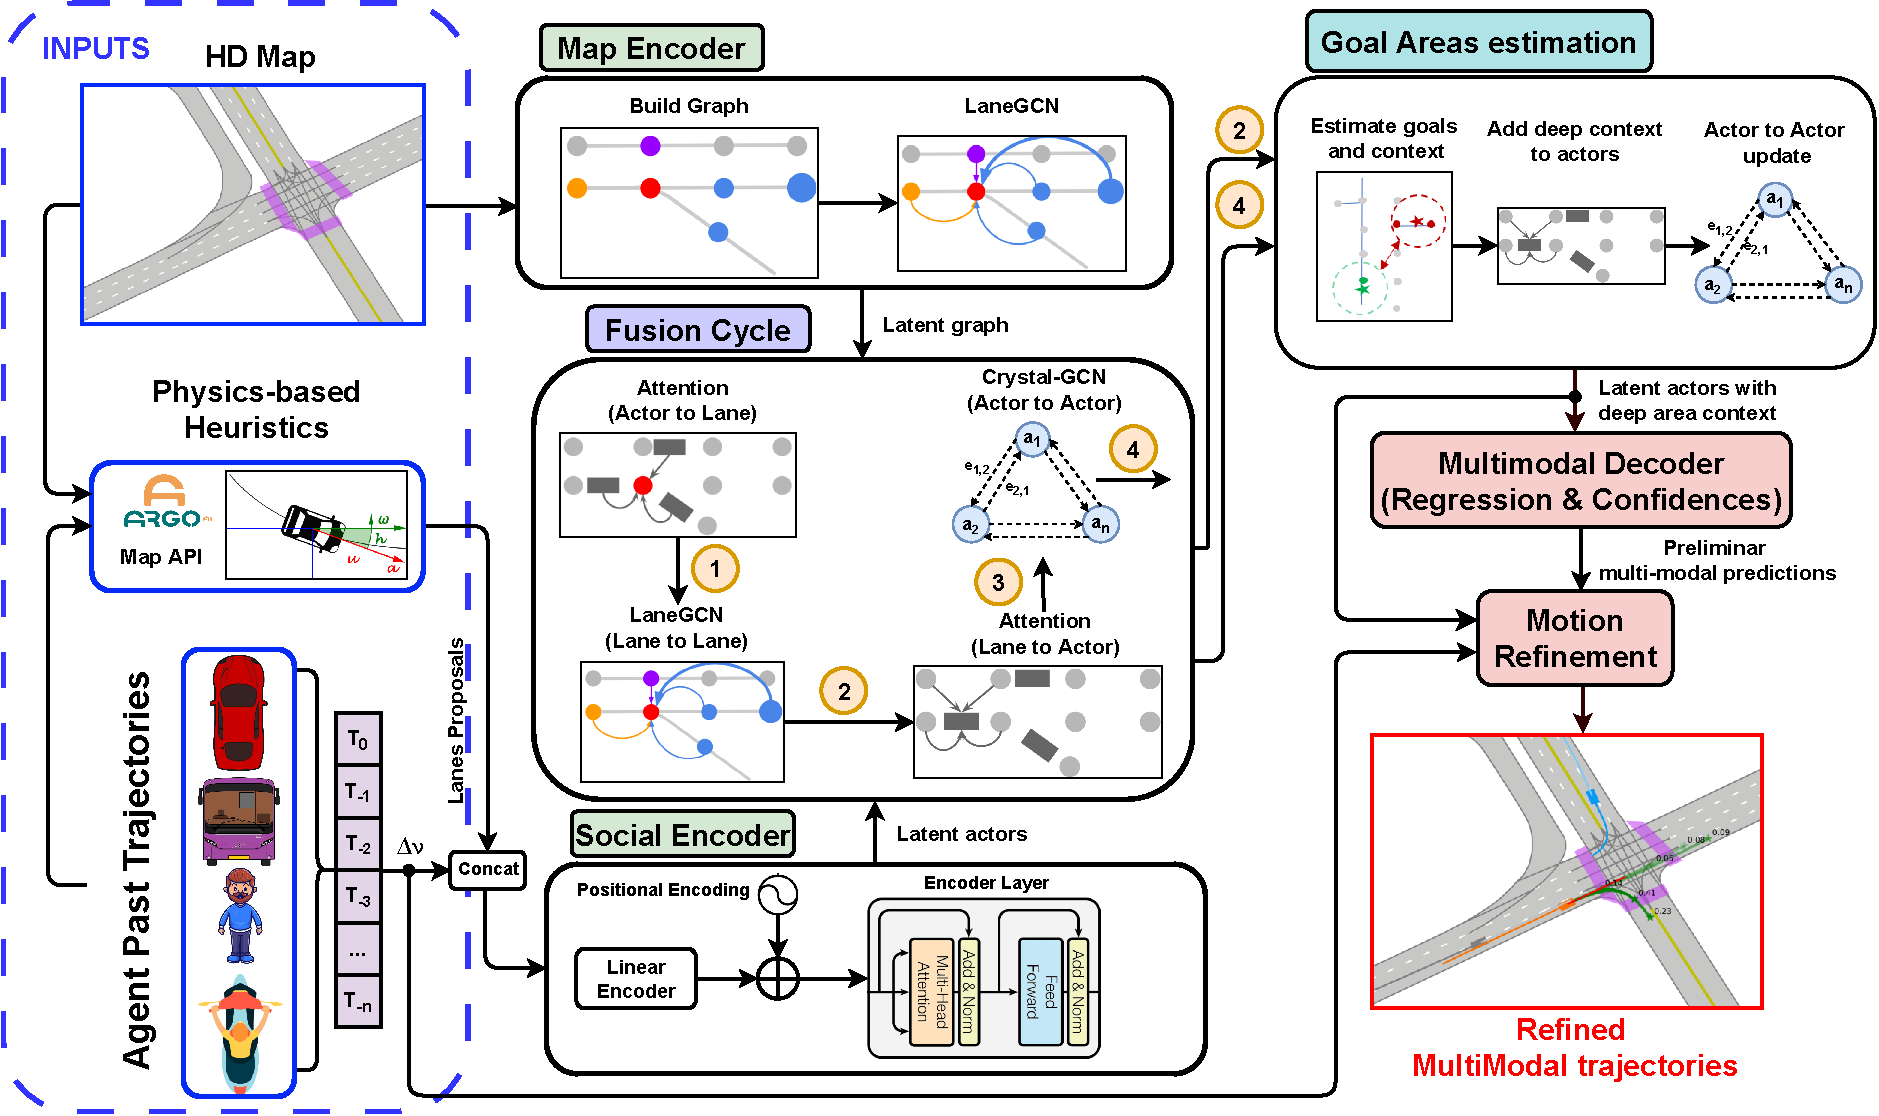
\includegraphics[width=\textwidth]{4_CVPR_2023.pdf}
	\caption[Overview of our Motion Prediction model including Fusion Cycle, Heuristic Proposals and Motion Refinement]{Overview of our Motion Prediction pipeline. We distinguish: 1) \textbf{Social Encoder}, which uses the agent past trajectories (relative displacements and additional metadata such as the type (\eg car, cyclist, pedestrian) and category, from less to more important) and the corresponding heuristic lane proposals to compute the social features, 2) \textbf{Map Encoder}, that constructs a lane graph from the HD Map and uses a LaneConv operator \cite{liang2020learning} to extract lane node features, 3) \textbf{Fusion Cycle}, responsible for fusing agents and map latent features, 4) \textbf{Goal Areas estimation}, to predict some goals and their surrounding  (area) features are aggregated to the agents, 5) \textbf{Multimodal Decoder}, which uses the latent actors with deep area context to generate reliable multi-modal predictions and 6) \textbf{Motion Refinement}, in charge of enhancing the quality of the future trajectories taking into account the past trajectories, actors latent features and preliminary predicted trajectories.}
	\label{fig:4_CVPR_2023}
\end{figure}

\subsection{Preprocessing of past trajectories and heuristic proposals}
\label{subsec:4_improving_efficiency_preprocessing}

The social preprocessing step proposed in this model is slightly different to our previous methods where we only considered those agents that have information over the full history horizon. Now, given the complexity of Argoverse 2, an agent that recently appeared in the scene, even if it was not observed over the whole full sequence spectrum, or even it was occluded for a few timestamps, it can be really relevant to determine the future behaviour of another agent. To this end, as proposed by multiple methods \cite{liang2020learning, schmidt2022crat}, we consider all agents that are observable at \textit{t=0}, handling those agents that are not observed over the full sequence spectrum (observation length = \textit{$obs_{len}$} + prediction length = \textit{$pred_{len}$}) by concatenating a binary flag $b_i^t$ that indicates if the agent is padded or not. On top of that, we only consider the dynamic agents of the scene (vehicles, pedestrians, motorcyclists, cyclists and buses) and discard unknown or static objects (background, construction or riderless bicycle), since dynamic (which can be stopped or not) are the most relevant for the \ac{MP} task. Given these final agents, we follow the same principles of translation and rotation invariant, as well as relative displacements, to compute the input past trajectories. On top of that, we additionally compute and codify the object type (bus, pedestrian, vehicle, cyclist) and agent importance (unscored, scored and focal track) as additional metadata. As described by Argoverse 2, each track is assigned one of the following labels, which dictate scoring behavior in the Argoverse 2 challenges:

\begin{enumerate}
	\item Track fragment: Lower quality track that may only contain a few timestamps of observations.
	\item Unscored track: Unscored track used for contextual input.
	\item Scored track: High-quality tracks relevant to the agent.
	\item Focal track: The primary track of interest in a given scenario - scored in the single-agent prediction challenge.
\end{enumerate}

We can appreciate how, in addition to the attention mechanisms of the model which are responsible of computing the most relevant features, the aforementioned track category serves as a good guidance as preliminary information to refer the importance of a specific agent with respect to another one.

In terms of physical information, we aim to increase the number of features of the HD Map as well as its corresponding interactions with the social features. Then, we focus on \textbf{Graph-based} methods \cite{zeng2021lanercnn} which construct graph-structured representations from the HD maps, which preserve the connectivity of lanes, and therefore the geometry of the scene. VectorNet \cite{gao2020vectornet} is one of the first works in this direction, where the authors propose to encode map elements and actor trajectories as polylines and then use a global interactive graph to fuse map and actor features. We find especially related LaneGCN \cite{liang2020learning}, a method that constructs a map node graph and proposes a novel graph convolution. In that sense, we follow the same principles than these well-established baselines by adopting simple form of vectorized map data as our representation of HD maps. In this case, the map data is represented as a set of polylines (lanes) and
their connectivity, where each lane contains a centerline (sequence of 2D \ac{BEV} points), arranged following the lane direction. For any two lanes which are directly reachable, 4 types of connections are given: predecessor, successor, left neighbour and right neighbour.

Moreover, we propose the use of preliminary plausible area information in a similar way to the heuristic proposals illustrated in Section \ref{subsubsec:4_efficient_baselines_preprocessing_map}. We follow the same heuristic (filter the agent, calculate the future travelled distance by means a CA model, get all candidates within a bubble, given the agent last observation and Manhattan distance, etc) to compute the most plausible future centerlines for the corresponding agent. It must be considered that in Argoverse 2 the number of categories is modified to 5 (vehicles, pedestrians, motorcyclists, cyclists and buses) insteaf of only 1 (vehicle) in the case of most vehicle \ac{MP} datasets, including Argoverse 1. So, no centerlines proposals are considered (then, they are created virtually and padded as stated in previous sections) since we assume that pedestrians are not walking on the road, but on the pedestrian crossings or sidewalks. In future works we will work on integrating specific physical information depending on the object type as preliminary map features. Nevertheless, in this particular case, thanks to a more realistic representation of the HD map, we include additional metadata such as lane type (bus, bike, vehicle), presence of intersection (binary flag) or boundaries mark type (dash, solid, yellow), along with the aforementioned centerline relative displacements. 

\subsection{Social Encoder}
\label{subsubsec:4_improving_efficiency_social_encoder}

As terms of social encoding, in order to capture more complex features for subsequent features fusion and interaction, we initially adopted GANet \cite{wang2022ganet}, based on LaneGCN \cite{liang2020learning}, to encode motion history and scene context for its outstanding performance. In this backbone (given the aforementioned social input: translation and rotation invariant with respect to a target agent, and relative displacements), LaneGCN makes use of use a network with $3$ groups/scales of 1D convolutions 1D CNN to process the trajectory input for its effectiveness in extracting multi-scale features and efficiency in parallel computing. The output is a well-structured feature map, whose element at $t=0$ is used as the actor feature. The network has $3$ groups/scales of 1D convolutions. Then, a Feature Pyramid Network (FPN) \cite{lin2017feature} to fuse the multi-scale features, and apply another residual block to obtain the output tensor. Moreover, GANet applies an \ac{LSTM} network on FPN output features and use two identical parallel networks to enhance the motion history encoding.

Regarding this, we aimed to improve social encoding taking into account that in spite the fact that \acp{LSTM} became popular because they could solve the problem of vanishing gradients, they suffer from \textit{short-term memory} due to the vanishing gradient problem, as well as require a lot of resources to get trained and become ready for real-world applications. In particular, they need high memory-bandwidth because of linear layers present in each cell which the system usually fails to provide for. To solve that, we replace the motion encoder proposed by \cite{wang2022ganet} for a transformer encoder, which is faster than \ac{RNN}-based models as all the input is ingested once, decreasing the computational complexity. On the other hand, even though the preliminary lane proposals represent physical information, they are quite related to the future intentions of the social information. Then, as depicted in Figure \ref{fig:4_CVPR_2023}, we concatenate the agents past trajectories, additional social metadata and heuristic map proposals (including semantic and topological metadata), which is processed by a linear embedding. Then, positional encoding is added to the output embedding explicitly to retain the information regarding the order of past trajectories and future preliminar steps. Finally, these latent features feed the transformer encoder, leveraging the self-attention mechanism and positional encoding to learn complex and dynamic patterns from long-term time series data. 

\subsection{Map preprocessing and encoding}
\label{subsec:4_improving_efficiency_map_preprocessing_and_encoding}

In terms of physical context, we adopt MapNet \cite{liang2020learning} backbone to encode the scene context for its outstanding performance. %It learns good lane representations which are computationally efficient and preserve map topology. We use a multi-scale LaneConv network to encode the vectorized map data, which is consisted of lane centerlines and their connectivity. We construct a lane node graph from the map data. A lane node is a short lane segment between two consecutive points of the lane centerline, which is represented by the location (the averaged coordinates of its two endpoints) and the shape (the vector between its two endpoints). 
While other approaches encode the map as a raster image and apply 2D convolutions to extract features, MapNet consists of two steps:

\begin{itemize}
	\item Build a lane graph from vectorized map data
	\item Apply a LaneConv operator to the lane graph to output the map features
\end{itemize}

\begin{figure}[h] 
	\centering
	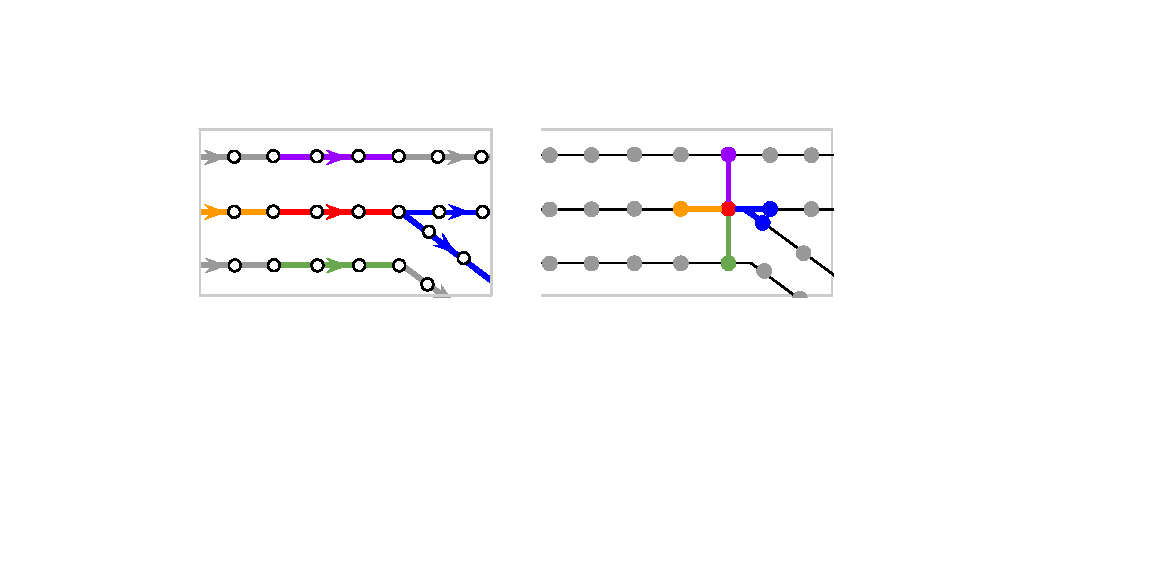
\includegraphics[width=0.8\textwidth]{4_lanegcn_map_representation.pdf}
	\caption{Lane graph construction from vectorized map data}
	Source: \textit{Learning lane graph representations for motion forecasting} \cite{liang2020learning}
	\label{fig:4_improving_efficiency_lanegcn_map_representation}
\end{figure}

As observed in Figure \ref{fig:4_improving_efficiency_lanegcn_map_representation}, the map data is represented as a set of lanes and their connectivity. Each lane contains a centerline, \ie, a sequence of 2D BEV points, which are arranged following the lane direction. For any two lanes which are directly reachable, $4$ types of connections are given: \textit{predecessor}, \textit{successor}, \textit{left neighbour} and \textit{right neighbour}. Given a lane $A$, its predecessor and successor are the lanes which can directly travel to $A$ and from $A$ respectively. Left and right neighbours refer to the  lanes which can be directly reached without violating traffic rules. This simple map format provides essential geometric and semantic information for \ac{MP}, as vehicles generally plan their routes by reference to lane centerlines and their connectivity. 

In order to conduct the Lane Graph construction, we first define a lane node as the straight line segment formed by any two consecutive points (grey circles in Figure \ref{fig:4_improving_efficiency_lanegcn_map_representation}) of the centerline. The location of a lane node is the averaged coordinates of its two end points. Following the  connections between lane centerlines, we also derive $4$ connectivity types for the lane nodes, \ie, \textit{predecessor}, \textit{successor}, \textit{left neighbour} and \textit{right neighbour}. For any lane node $A$, its predecessor and successor are defined as the neighbouring lane nodes that can travel to $A$ or from $A$ respectively. Note that one can reach the first lane node of a lane $l_{A}$ from the last lane node of lane $l_{B}$ if $l_{B}$ is the predecessor of $l_{A}$. Left and right neighbours are defined as the spatially closest lane node measured by $\ell_2$ distance on the left and on the right neighbouring lane respectively. We denote the lane nodes with $V \in \mathbb{R}^{N \times 2}$, where $N$ is the number of lane nodes and the $i$-th row of $V$ is the BEV coordinates of the $i$-th node. We represent the connectivity with $4$ adjacency matrices $\{A_i\}_{ i \in \{\text{pre}, \text{suc}, \text{left}, \text{right}\} }$, with $A_i \in \mathbb{R}^{N \times N}$. We denote $A_{i, jk}$, as the element in the $j$-th row and $k$-th column of $A_i$. Then  $A_{i, jk} = 1$ if node $k$ is an $i$-type neighbor of node $j$. 

\subsubsection{LaneConv Operator}
\label{subsubsec:4_improving_efficiency_lane_conv}

A natural operator to handle lane graphs is the graph convolution \cite{shuman2013emerging}.
The most widely used graph convolution operator \cite{kipf2016semi} is defined as $Y = LXW$, where $X \in \mathbb{R}^{N \times F}$ is the node feature, $W \in \mathbb{R}^{F \times O}$ is the weight matrix, and $Y \in \mathbb{R}^{N \times O}$ is the output. The graph Laplacian matrix $L \in \mathbb{R}^{N \times N}$ takes the form $L = D^{-1/2}(I + A)D^{-1/2}$, where $I$, $A$ and $D$ are the identity, adjacency and degree matrices respectively. $I$ and $A$ account for self connection and connections between different nodes. All connections share the same weight $W$, and the degree matrix $D$ is used to normalize the output. However, this vanilla graph convolution is inefficient in our case due to the following reasons. First, it is not clear what kind of node feature will preserve the information in the lane graphs. Second, a single graph Laplacian can not capture the connection type, \ie, losing the directional information carried by the connection type. Third, it is not straightforward to handle long range dependencies, \eg, akin dilated convolution, within this form of graph convolution. Motivated by these challenges, we introduce our novel specially designed operator for lane graphs, called \textit{LaneConv}.

\paragraph{Node Feature}

We first define the input feature of the lane nodes. Each lane node corresponds to a straight line segment of a centerline. To encode  all the lane node information, we need to take into account both the shape (size and orientation) and the location (the coordinates of the center) of the corresponding line segment. We parameterize the node feature as follows:

\begin{equation}
	\mathbf{x}_i = \text{MLP}_\text{shape} \left( \mathbf{v}_i^{\text{end}} - \mathbf{v}_i^{\text{start}} \right)
	+ \text{MLP}_{\text{loc}}\left(\textbf{v}_i\right)
	\label{eqn:node_feat}
\end{equation}

where $\text{MLP}$ indicates a multi-layer perceptron and the two subscripts refer to shape and location, respectively.  $\textbf{v}_i$ is the location of the $i$-th lane node, \ie, the center between two end points, $\mathbf{v}_i^{\text{start}}$ and $\mathbf{v}_i^{\text{end}}$ are the BEV coordinates of the node $i$'s starting and ending points, and $\mathbf{x}_i$ is the $i$-th row of the node feature matrix $X$, denoting the input feature of the $i$-th lane node.

\paragraph{LaneConv}

The node feature above only captures the local information of a line segment.
To aggregate the topology information of the lane graph at a larger scale,
we design the following LaneConv operator:

\begin{equation}
	Y = X W_0 + \sum_{i \in \{ \text{pre}, \text{suc}, \text{left}, \text{right} \}} {A_{i} X W_{i}}
	\label{eqn:laneconv}
\end{equation}

where $A_{i}$ and $W_i$ are the adjacency  and the weight matrices corresponding to the $i$-th connection type respectively. Since we order the lane nodes from the start to the end of the lane, $A_{\text{suc}}$ and $A_{\text{pre}}$ are matrices obtained by shifting the identity matrix one step towards upper right (non-zero superdiagonal) and lower left (non-zero subdiagonal). $A_{\text{suc}}$ and $A_{\text{pre}}$ can propagate information from the forward and backward neighbours whereas $A_{\text{left}}$ and $A_{\text{right}}$ allow information to flow from the cross-lane neighbours. It is not hard to see that our LaneConv builds on top of the general graph convolution and encodes more geometric (\eg, connection type/direction) information.

\paragraph{Dilated LaneConv}

Since motion forecasting models usually predict the future trajectories of actors with a time horizon of several seconds, actors with high speed could have moved a long distance.
Therefore, the model needs to capture the long range dependency along the lane direction for accurate prediction. In regular grid graphs, a dilated convolution operator \cite{yu2015multi} can effectively capture the long range dependency by enlarging the receptive field. Inspired by this operator, we propose the \textit{dilated LaneConv} operator to achieve a similar goal for irregular graphs. 

In particular, the $k$-dilation LaneConv operator is defined as follows:
 
\begin{equation}
	Y = XW_0 + A_{\text{pre}}^k X W_{\text{pre},k} + A_{\text{suc}}^k X W_{\text{suc},k}
	\label{eqn:dilated_laneconv}
\end{equation}

where $A_{\text{pre}}^k$ is the $k$-th matrix power of $A_{\text{pre}}$. 
This  allows us to directly propagate information along the lane for $k$ steps, with $k$ a hyperparameter. Since $A_{\text{pre}}^k$ is highly sparse, one can efficiently compute it using sparse matrix multiplication. Note that the dilated LaneConv is only used for predecessor and successor, as the long range dependency is mostly along the lane direction.

\subsubsection{LaneGCN}\label{sec:LGN}
\label{subsubsec:4_improving_efficiency_lanegcn}

\begin{figure}[t]                               
	\begin{center}
		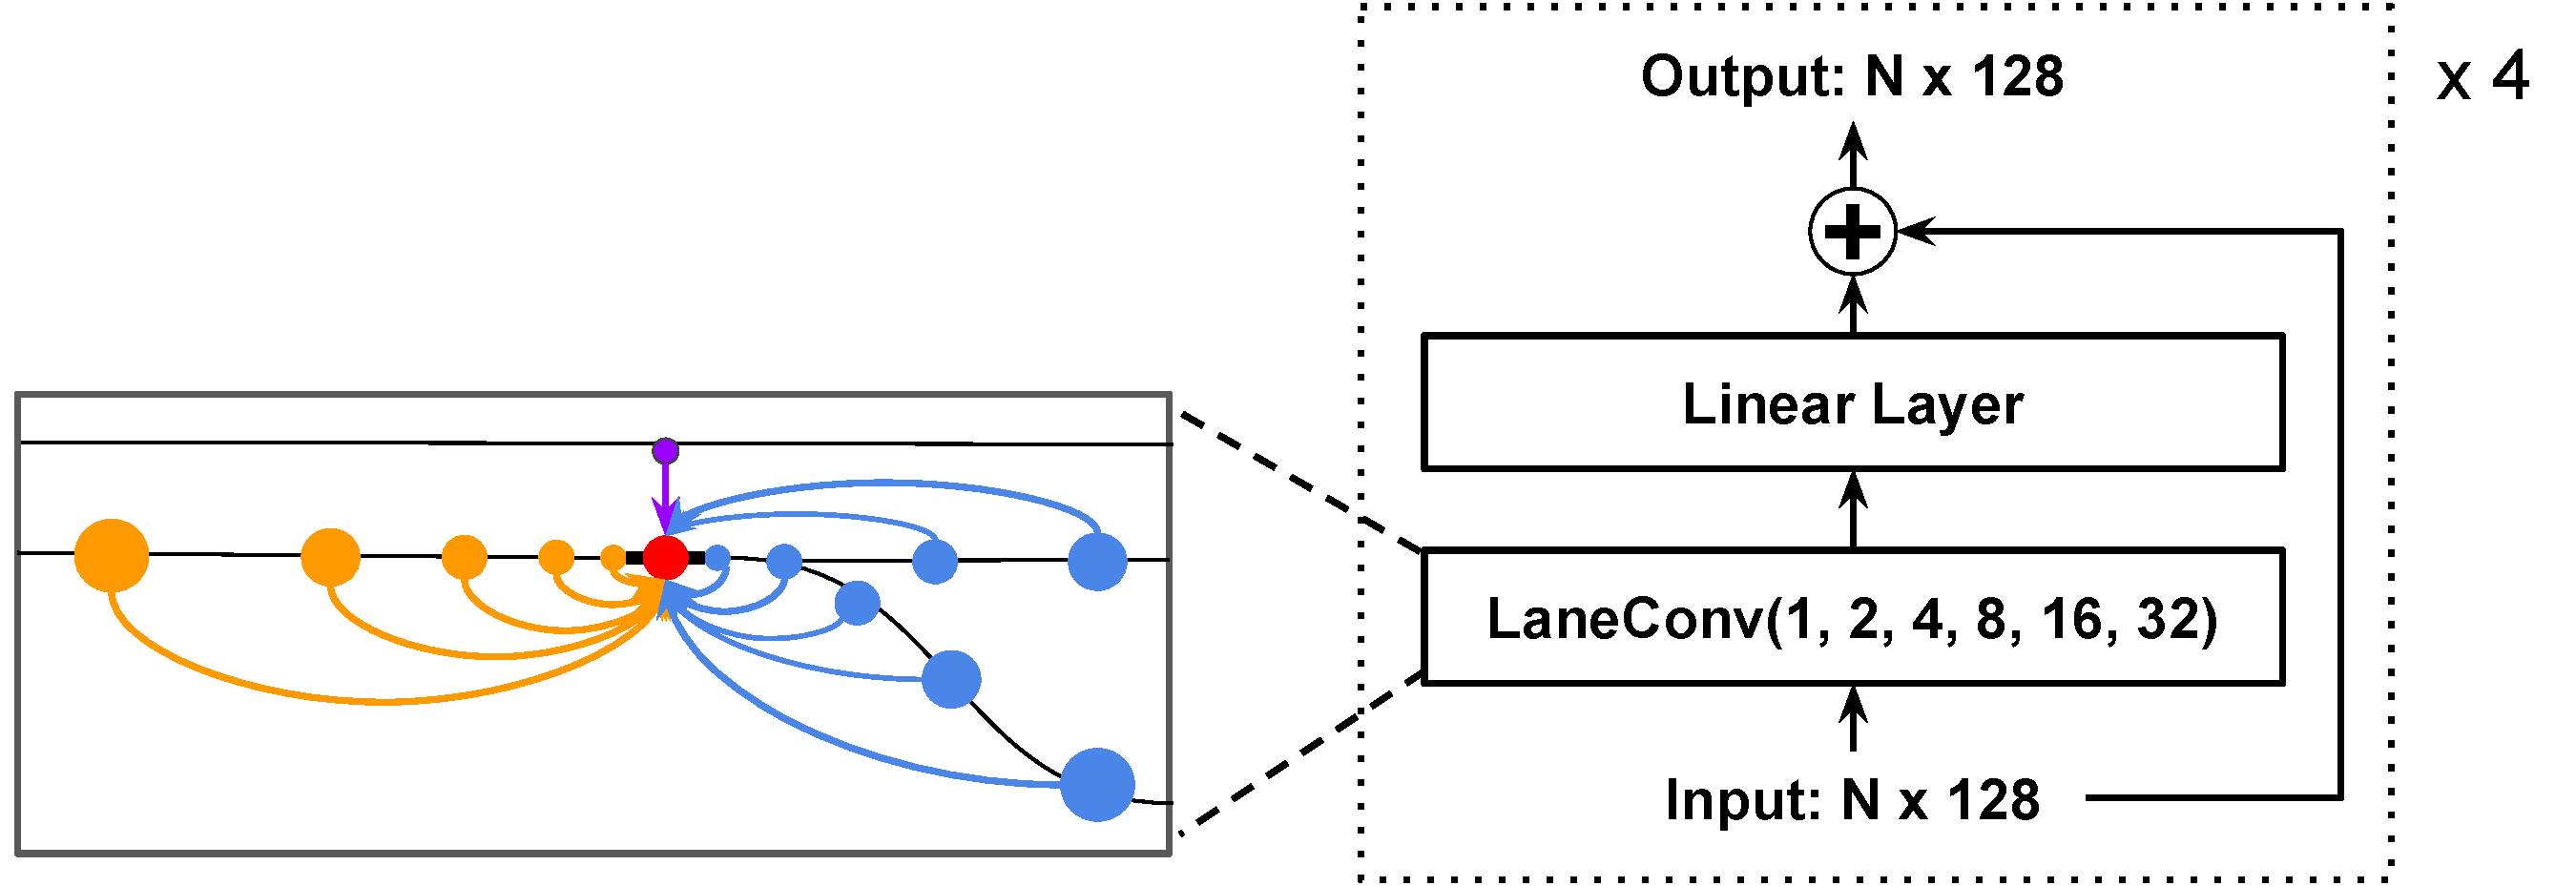
\includegraphics[width=0.8\linewidth]{4_lanegcn_scheme.pdf}
	\end{center}
	\caption[LaneGCN architecture]{LaneGCN architecture. LaneGCN is a stack of 4 multi-scale LaneConv residual blocks, each of which consists of a LaneConv(1,2,4,8,16,32) and a linear layer with a residual connection.}
	Source: \textit{Learning lane graph representations for motion forecasting} \cite{liang2020learning}
	\label{fig:4_improving_efficiency_lanegcn}
\end{figure}
	
Based on the dilated LaneConv, we further propose a multi-scale LaneConv operator and use it to build our LaneGCN.
Combining Eq. (\ref{eqn:laneconv}) and (\ref{eqn:dilated_laneconv}) with multiple dilations, we get a multi-scale LaneConv operator with $C$ dilation sizes as follows
\begin{equation}\label{eqn:dilated_laneconv_final}
	Y = XW_0 + \sum_{i \in \{ \text{left}, \text{right} \}} {A_{i} X W_{i}}
	+ \sum_{c=1}^{C} {\left( A_{\text{pre}}^{k_{c}} X W_{\text{pre},k_{c}} + A_{\text{suc}}^{k_{c}} X W_{\text{suc},k_{c}} \right)},
\end{equation}
where $k_c$ is the $c$-th dilation size. We denote  $\text{LaneConv}(k_1, \cdots, k_C)$ this multi-scale layer. 

\subsection{Enhanced Actor-Map Fusion Cycle}
\label{subsubsec:4_improving_efficiency_enhanced_fusion_cycle}

Once both the map and social latent features are computed, we obtain a 2D feature matrix $X$ where each row $X_i$ indicates the feature of the $i$-th actor, and a 2D matrix $Y$ where each row $Y_i$ indicates the feature of the $i$-th lane node. Then, we make use of the well-established actor-map fusion cycle \cite{liang2020learning} (also referred as FusionNet in the literature) that transfers and aggregates feature among actors and lane nodes. The behaviour of an actor strongly depends on its context, \ie, other actors and the map. Although the interactions between actors has been explored by previous work, the interactions between the actors and the map, and map conditioned interactions between actors have received much less attention. FusionNet makes use of spatial attention and LaneGCN to capture a complete set of actor-map interactions, as observed in Figure \ref{fig:4_CVPR_2023}.

FusionNet makes use of a stack of four fusion modules to capture all information flows between actors and lane nodes, \ie, (1) Actors to Lanes (A2L), (2) Lanes to Lanes (L2L), (3) Lanes to Actors (L2A) and (4) Actors to Actors (A2A). This order is not coincidence. Assuming several agents are on the road and all of them have a web service that provides detailed information about geographical regions and sites worldwide (\eg, Google Maps):

\begin{itemize}
	\item First, agents introduce their real-time traffic information to lane nodes, such as blockage, presence of an accident, etc. In other words, the HD map information is updated with the traffic information of the agents.
	\item The HD map information of a particular node is propagated to the immediate neighbours, in such a way ...
	\item ... Further agents are updated with the information of surrounding map nodes, which were previously updated by neighboring nodes.
	\item Finally, A2A concludes the actor-map fusion cycle handling the interactions between actors and produces the output actor features.
	
\end{itemize}

We implement L2L using another LaneGCN, which has the same architecture as the one used in our MapNet. Regarding the A2L, L2A and A2A modules, \cite{liang2020learning} applies a spatial attention layer as defined in Section \ref{subsec:3_attention}. Taking the first module (A2L) as en example, given an actor node $i$, we aggregate the features from its context lane nodes $j$ as follows:

\begin{equation}
	\mathbf{y}_i = \mathbf{x}_i W_0 + \sum_j \phi ( \text{concat} (\mathbf{x}_i, \Delta_{i,j}, \mathbf{x}_j) W_1) W_2
	\label{equ:attention}
\end{equation}

where $\mathbf{x}_i$ represents the feature of the $i$-th node, $W$ a weight matrix, $\phi$ the composition of layer normalization and ReLU, and $\Delta_{ij} = \text{MLP}(\mathbf{v}_j - \mathbf{v}_i)$, where $\mathbf{v}$ denotes the node location.

The context nodes are defined to be the lane nodes whose $\ell_2$ distance from the actor node $i$ is smaller than a threshold. Each of A2L, L2A and A2A has two residual blocks, which consist of a stack of the proposed attention layer and a linear layer, as well as a residual connection. 

Nevertheless, as observed in our model (Figure \ref{fig:4_CVPR_2023}), once implemented FusionNet to compute actor-map interactions, we substitute the final module that models Actor to Actor interactions with a Graph Convolution Operator (GCN), inspired in our previous proposed efficient baselines (Figure \ref{fig:4_TITS_2023}). Further results (Section \ref{sec:5_motion_prediction_datasets}) will illustrate that replacing the final spatial attention among agents by an efficient graph operator preserves global agent interaction while enhances the whole model in terms of computational complexity and inference time.

\begin{comment}
	\subsection{Decoding Module}
	
	\subsubsection{Goals Prediction and Filtering}
	
	\paragraph{Goals predictions}
	
	Since we use GANet~\cite{wang2022ganet} as baseline method, we follow the same approach to predict goal points \ie potential destination points for each agent in the scene.
	
	We train the goal predictor as~\cite{wang2022ganet} -following the same network architecture- using a combination of classification loss and regression loss. Given $E$ predicted goals, we find a positive goal $\hat{e}$ that has the minimum $\mathcal{L}_2$ distance \emph{w.r.t} the ground truth trajectory's endpoint --- making the predicted goal close to the actual goal as much as possible.
	
	This goal prediction module serves to locate goal areas (\eg plausible areas of movement within the lanes). In practice, a drivers behaviour is highly multi-modal and stochastic \eg the driver can stop, go ahead, turn left or right when approaching an intersection, or accelerate. Therefore, we try to make a multiple-goals prediction. 
	
	\paragraph{GoICrop}
	
	Following GANet~\cite{wang2022ganet}, we choose the predicted goal with the highest confidence among $E$ goals as an anchor. This anchor, by definition, approximates the destination of the agent with the highest probability based on its past trajectories and the scene context.
	
	Hence, we use the predicted anchors and apply a GoICrop~\cite{wang2022ganet} filtering to implicitly model actors interactions in the future. This ROI (Regions of Interest) filter allows to select the goal points (anchors) for each agent, considering the their probable interations.
	
	\subsubsection{Trajectory Prediction}
	
	Finally, we take the updated actor features $X$ as input to predict $K$ final future trajectories and their confidence scores. Following our baseline~\cite{wang2022ganet} we use a standard multi-modal decoder  with one regression branch estimating the trajectories, and one classification branch predicting the corresponding confidences.
\end{comment}

\subsection{Goal prediction}
In stage two, we predict possible goals for the $i$-th actor based on $X_i$. 
We apply intermediate supervision and calculate the smooth L1 loss between the best-predicted goal and the ground-truth trajectory's endpoint to backpropagate, making the predicted goal close to the actual goal as much as possible. 
The goal prediction stage serves as a predictive test to locate goal areas, which is different from goal-based methods using the predicted goals as the final predicted trajectories' endpoint. 
In practice, a driver's driving intent is highly multi-modal. 
For example, he or she may stop, go ahead, turn left, or turn right when approaching an intersection. 
Therefore, we try to make a multiple-goals prediction. 
We construct a goal prediction header with two branches to predict $E$ possible goals $G_{n,end} =\{g_{n,end}^e\}_{e \in [0,E-1]}$ and their confidence scores $    C_{n,end} = \{c_{n,end}^e\}_{e \in [0,E-1]}$, 
where $g_{n,end}^e$ is the $e$-th predicted goal coordinates and $c_{n,end}^e$ is the $e$-th predicted goal confidence of the $n$-th actor.

We train this stage using the sum of classification loss and regression loss.
Given $E$ predicted goals, we find a positive goal $\hat{e}$ that has the minimum Euclidean distance with the ground truth trajectory's endpoint. 
For classification, we use the max-margin loss:
\begin{equation}
	L_{cls\_end}=\frac{1}{N(E-1)}\sum_{n=1}^N\sum_{e\neq \hat{e}}{max(0,c^e_{n,end}+\epsilon -c^{\hat{e}}_{n,end})}
\end{equation}
where $N$ is the total number of actors and $\epsilon =0.2$ is the margin. The margin loss expects each goal to capture a specific pattern and pushes the goal closest to the ground truth to have the highest score.
For regression, we only apply the smooth L1 loss to the positive goals:
\begin{equation}
	L_{reg\_end}=\frac{1}{N}\sum_{n=1}^N{reg(g_{n,end}^{\hat{e}}-a^{*}_{n,end})}
\end{equation}
where $a^{*}_{n,end}$ is the ground truth BEV coordinates of the $n$-th actor trajectory's endpoint, $reg(z) = \sum_id(z_i)$, $z_i$ is the $i$-th element of $z$, and $d(z_i)$ is a smooth L1 loss.

Additionally, we also try to add a "one goal prediction" module at each trajectory's middle position aggregating map features to assist the endpoint goal prediction and the whole trajectory prediction.
Similarly, we apply a residual MLP to regress a middle goal $g_{n,mid}$ for the $n$-th actor. 
The loss term for this module is given by:
\begin{equation}
	L_{reg\_mid} = \frac{1}{N}\sum_{n=1}^N {reg(g_{n,mid}-a^*_{n,mid})}
\end{equation}
where $a^*_{n,mid}$ is the ground truth BEV coordinates of the $n$-th actor trajectory's middle position.

The total loss at the goal prediction stage is:
\begin{equation}
	L_{1} = \alpha_1 L_{cls\_end} + \beta_1 L_{reg\_end} +\rho_1 L_{reg\_mid}
\end{equation}
where $\alpha_1 = 1$, $\beta_1 = 0.2$ and $\rho_1 = 0.1$.

\subsection{GoICrop}
We choose the predicted goal with the highest confidence among $E$ goals as an anchor. This anchor is the approximate destination with the highest possibility that the actor may reach based on its motion history and driving context.
Because the actors' motion is highly uncertain, we crop maps within 6 meters of the anchor as the goal area of interest, which relaxes the strict goal prediction requirement. The actual endpoint is more likely to appear in candidate areas compared with being hit by scattered endpoint predictions.
Moreover, the actor's behavior highly depends on its destination area's context, i.e., the maps and other actors. Although previous works have explored the interactions between actors, the interactions between actors and maps in goal areas and the interactions among actors in the future have received less attention. 
Thus, we retrieve the lane nodes in goal areas and apply a GoICrop module to aggregate these map node features as follows:
\begin{equation}
	x'_i = \phi_1(x_iW_0+\sum_j\phi_2(concat(x_iW_1,\Delta_{i,j},y_j)W_2))W_3
	\label{att}
\end{equation}
where $x_i$ is the feature of $i$-th actor and and $y_j$ is the feature of $j$-th lane node, $W_i$ is a weight matrix, $\phi_i$ is a layer normalization with ReLU function, and $\Delta_{i,j}=\phi(MLP(v_i-v_j))$, where $v_i$ denotes the anchor's coordinates of $i$-th actor and $v_j$ denotes the $j$-th lane node's coordinates. 
GoICrop serves as spatial distance-based attention and updates the goal area lane nodes' features back to the actors. We transpose $x_i$ with $W_1$ as a query embedding. The relative distance feature between the anchor of $i$-th actor and $j$-th lane node are extracted by $\Delta_{i,j}$. Then, we concatenate the query embedding, relative distance feature, and lane node feature. An $MLP$ is employed to transpose and encode these features. Finally, the goal area features are aggregated for $i$-th actor.

Previous motion forecasting methods usually focus on the interactions in the observation history. 
However, actors will interact with each other in the future to follow driving etiquette, such as avoiding collisions. 
Since we have performed predictive goal predictions and gotten possible goals for each actor, our framework can model the actors' future interactions.
Hence, we utilize the predicted anchor positions and apply a GoICrop module as equation~\ref{att} to implicitly model actors' interactions in the future. We consider the other actors whose future anchor's distance from the anchor of $i$-th actor is smaller than 100 meters. In this case, $y_j$ in equation~\ref{att} denotes the features of $j$-th actor, $v_i$ denotes the anchor's coordinates of $i$-th actor, and $v_j$ denotes the anchor's coordinates of $j$-th actor in $\Delta_{i,j}=\phi(MLP(v_i-v_j))$.

\subsection{Decoding module}
In order to get the future trajectories with corresponding scores, as observed in Figure \ref{fig:4_CVPR_2023}, we take the updated actor features $X$ as input to predict $K$ final future trajectories and their confidence scores in stage three. 
Specifically, we construct a two-branch multi-modal prediction header similar to the goal prediction stage, with one regression branch estimating the trajectories and one classification branch scoring the trajectories.
For each actor, we regress $K$ sequences of BEV coordinates 
$    A_{n,F}=\{(a_{n,1}^k,a_{n,2}^k,...,a_{n,T}^k)\}_{k \in [0,K-1]}$,
where $a_{n,t}^k$ denotes the $n$-th actor's future coordinates of the $k$-th mode at $t$-th step. 
For the classification branch, we output $K$ confidence scores $    C_{n,cls} = \{c_n^k\}_{k \in [0,K-1]}
$ corresponding to $K$ modes.
We find a positive trajectory of mode $\hat{k}$, whose endpoint has the minimum Euclidean distance with the ground truth endpoint.

For classification, we use the margin loss  $L_{cls}$ similar to the goal prediction stage. 
For regression, we apply the smooth L1 loss on all predicted steps of the positive trajectories:
\begin{equation}
	L_{reg}=\frac{1}{NT}\sum_{n=1}^N\sum_{t=1}^T{reg(a_{n,t}^{\hat{k}}-a^{*}_{n,t})}
\end{equation}
where $a^{*}_{n,t}$ is the $n$-th actor's ground truth coordinates.

To emphasize the importance of the goal, we add a loss term stressing the penalty at the endpoint:
\begin{equation}
	L_{end}=\frac{1}{N}\sum_{n=1}^N{reg(a_{n,end}^{\hat{k}}-a^{*}_{n,end})}
\end{equation}
where $a^{*}_{n,end}$ is the $n$-th actor's ground truth endpoint coordinates and $a_{n,end}^{\hat{k}}$ is the $n$-th actor's predicted positive trajectory's endpoint.

The loss function for training at this stage is given by:
\begin{equation}
	L_{2} = \alpha_2 L_{cls} + \beta_2 L_{reg} + \rho_2 L_{end}
\end{equation}
where $\alpha_2=2$, $\beta_2=1$ and $\rho_2=1$.

\subsection{Motion refinement}
\label{subsec:refinement}

A second-stage motion refinement, as proposed by \cite{liu2023laformer}, is introduced to further explore the temporal consistency for predicting more accurate future trajectories. The goal is to reduce the offset between ground truth trajectory $Y$ and predicted trajectory $\hat{Y}$. We define this offset as $\Delta{Y} = Y - \hat{Y}$. In this stage, we leverage three sources of information: 1. Preliminary predictions computed in the decoding module, 2. Prior latent information to the decoding module and 3. Past observations. Using this approach, an MLP model is trained to minimize the offset by predicting a residual $R$ that is added to the original trajectory \ie we use $L_2$ loss to optimize the offset as follows:

\begin{equation}
	\label{eq:5_pose_error}
	\mathcal{L}_\text{off}= ||{Y} - \hat{Y} - \hat{R}||_2 = ||\Delta{Y} - \hat{R}||_2.
\end{equation}

Furthermore, we use a cosine function, denoted by Equation \ref{eq:5_cosine_error}, to explicitly aid the model in learning the turning angle from the last observed position. It measures the difference between the ground truth angle $\theta_{t}= \text{arctan2}(Y_{t}-{X}_{0})$ and the predicted angle $\hat{\theta}_{t}= \text{arctan2}(\hat{Y}_{t}-{X}_{0})$:

\begin{equation}
	\mathcal{L}_{\text{angle}}=\frac{1}{t_{f}}\sum^{t_{f}}_{t=1}-cos(\hat{\theta}_{t}-\theta_{t})
	\label{eq:poseerror}
\end{equation}

Note that this method can be applied to the pre-trained model from previous stages, which is completely functional, as the main function is to improve the output trajectories.

\section{Summary}

In this chapter we have proposed several predictive techniques for scene understanding in the field of \ac{AD}. First of all, we propose SmartMOT, a simple-yet-powerful pipeline that fuses the concepts of tracking-by-detection and HD map information to design a real-time and power-efficient \ac{MOT} and \ac{MP} pipeline to track and predict the future trajectories of only the most relevant obstacles around the ego-vehicle. Then, the thesis focuses on applying \ac{DL} to obtain rich features from the context (both in terms of social and map information) and subsequently predict the future trajectories of certain agents in the scene by means a multimodal prediction, where confidences are considered. While focusing on efficiency and interpretability, we progressively incorporate more information and \ac{SOTA} mechanisms (\ac{GAN}, \ac{GNN}, Attention), as well as specific preprocessing steps, heuristic and operations for \ac{MP} to help the models compute plausible predictions in real-time.

We hope that our proposals can serve as a solid baseline on which others can build on to advance the state-of-the-art in fusing perception data and map information to perform real-time motion prediction and decision-making evaluation in arbitrarily complex urban scenarios. 

